\documentclass{VUMIFPSkursinis}
\usepackage{algorithmicx}
\usepackage{algorithm}
\usepackage{algpseudocode}
\usepackage{amsfonts}
\usepackage{amsmath}
\usepackage{bm}
\usepackage{caption}
\usepackage{biblatex}
\usepackage{color}
\usepackage{float}
\usepackage{graphicx}
\usepackage{listings}
\usepackage{subfig}
\usepackage{wrapfig}
\usepackage{multirow}
\usepackage{longtable}
\usepackage{array,makecell}
\usepackage{enumitem}

% Titulinio aprašas
\university{Vilniaus universitetas}
\faculty{Matematikos ir informatikos fakultetas}
\department{Programų sistemų katedra}
\papertype{Programų sistemų inžinerija}
\title{Keleivių kontrolės paieškos programėlė}
\titleineng{AVOID A TICKET}
\status{2 kurso 5 grupės studentai}
\author{Elena Reivytytė}
\secondauthor{Matas Šilinskas}
\thirdauthor{Kasparas Taminskas}
\fourthauthor{Aidas Vaikšnoras}
\fifthauthor{Tadas Žaliauskas}
\supervisor{dr. Vytautas Valaitis}
\date{Vilnius – \the\year}

% Nustatymai
% \setmainfont{Palemonas}   % Pakeisti teksto šriftą į Palemonas (turi būti įdiegtas sistemoje)
\bibliography{bibliografija}

\begin{document}
\maketitle

\sectionnonum{Anotacija}
Šis dokumentas skirtas Vilniaus universiteto Programų sistemų 2 kurso Programų sistemų inžinerijos II modulio pirmąjam (reikalavimai ir ICONIX užduočių tekstai, sąsajos maketai ), antrąjam (robastiškumo diagramos, preliminari peržiūra, techninė architektūra) ir trečiajam (detalaus dizaino įgyvendinimas) laboratoriniams darbams atlikti.

\tableofcontents

\sectionnonum{Įvadas}
\noindent
\textbf{Programų sistemos pavadinimas}\\
Programėlės pavadinimas AvoidATicket išvertus iš anglų kalbos reiškia „Nepirk bilieto be reikalo“\\
\textbf{Dalykinė sritis}\\
Programėle, kurioje viešojo transporto keleiviai gali dalintis informacija apie vykdomas viešojo transporto bilietų patikras.\\
\textbf{Probleminė sritis}\\
Programėlė yra skirta padėti klientams sutrumpinti kelionių laiką parodant, kuriose vietose keleivių kontrolė tikrina autobusus.\\
\textbf{Vartotojas}\\
Klientas - bet kokio amžiaus žmogus, kuris turi išmanųjį telefoną ir naudojasi miestinių autobusų teikiamomis paslaugomis.\\
\textbf{Darbo pagrindas}\\
Tikslas ištirti rinką galimam programėlės vystymui. Taip pat programėlės projektavimas teoriniame lygmeny siekiant supaprastint programavimo darbus.\\
\textbf{Darbo pagrindas}\\
\begin{tabular}{lr}
   Elena Reivytytė & 20\% \\
   Aidas Vaikšnoras & 20\% \\
   Kasparas Taminskas & 20\% \\
   Tadas Žaliauskas & 20\% \\
   Matas Šilinskas & 20\% \\
\end{tabular}
\\
\textbf{Naudojama informacija}\\
Šis dokumentas rengiamas pagal PSI II kurso laboratorinių darbų reikalavimus, išdėstytus~\ref{petrauskas} šaltinyje. Visas kurso turinys susijęs su ICONIX programų kūrimo proceso metodologija,
kuri detaliai aprašoma~\ref{iconix} knygoje. UML specifika aprašoma~\ref{uml} ir~\ref{omguml} resursuose.

\section{Poreikiai}
\begin{enumerate}[itemsep=-2mm]
	\item Vartotojas gali prisijungti, atsijungti ir registruotis prie programėlės.
	\item Vartotojas turi galimybę prisijungti naudojantis “Facebook” paskyra.
	\item Vartotojas gali keisti registracijos metu įvestus duomenis: vardą, pavardę, el. paštą, slaptažodį, prisijungimo vardą.
	\item Vartotojas gali pridėti žymeklį, nurodantį vietą, kurioje yra kontrolė netoliese nuo jo esančiu atstumu (1500 metrų).
	\item Vartotojas balsuodamas gali patvirtinti arba paneigti, kad žymeklio vietoje stovi keleivių kontrolė.
	\item Vartotojas gali sekti dominančius transporto maršrutus ir realiu laiku stebėti, kuriose maršruto stotelėse stovi kontrolė. 
	\item Vartotojas gali peržiūrėti kitų vartotojų padėtus žymeklius. 
	\item Vartotojas gali palikti komentarą apie žymeklį. 
	\item Vartotojas gali perskaityti D.U.K. programėlėje.
	\item Vartotojas gali užduoti klausimą.
	\item Administratorius gali keisti kiekvieno vartojo vardą, pavardę, el. paštą, slaptažodį, prisijungimo vardą.
	\item Administratorius gali pridėti naują vartotoją ir administratorių.
	\item Programėle turi būti anglų kalba. 
	\item Padėti žymekliai rodomi tik tam tikrą laiko tarpą.
	\item Administratorius gali ištrinti bet kurį vartotojo pažymėtą žymeklį.
	\item Išjungus programėlę, vartotojas liekas prisijungęs.
\end{enumerate} 

\section{Reikalavimai}
Šiame skyriuje pateikiami sistemos funkciniai ir nefunkciniai reikalavimai, sudaryti pagal užsakovo nurodytus poreikius.
\subsection{Funkciniai reikalavimai }
Šiame skyriuje pateikiami sistemos funkciniai reikalavimai, t.y. pagrindinės sistemos atliekamos funkcijos, konkretūs jų aprašymai.

\newcounter{frcount}
\newcommand\rownumberfr{\stepcounter{frcount}\arabic{frcount}}

\begin{longtable}{ | >{\centering}m{2cm} | m{10cm} | >{\centering}m{2.5cm} | } \caption{Funkciniai reikalavimai.} \endhead \hline
\multicolumn{3}{ |l| }{\textbf{Funkciniai reikalavimai:}} \tabularnewline \hline
\textbf{Numeris} & \centering{\textbf{Reikalavimas}} & \textbf{Svarba} \tabularnewline \hline

FR\rownumberfr & Įsijungęs programėlę, vartotojas gali:
						\begin{enumerate}[itemsep=-2mm]
							\item registruotis
							\item prisijungti
							\item neteisingai įvedęs duomenis, vartotojas gali pasitaisyti
						\end{enumerate}
				\textit{Žr. skyrius poreikiai, 1 punktas} & Būtina\tabularnewline \hline

FR\rownumberfr & Prisijungęs vartotojas gali atsijungti.\newline \textit{Žr. skyrius poreikiai, 1 punktas} & Būtina\tabularnewline \hline
FR\rownumberfr & Vartotojas gali prisijungti naudodamas “Facebook” paskyrą.\newline \textit{Žr. skyrius poreikiai, 2 punktas} & Būtina\tabularnewline \hline
FR\rownumberfr & Savo paskyroje vartotojas gali keisti:
						\begin{enumerate}[itemsep=-2mm]
							\item slaptažodį
							\item vardą
							\item pavardę
							\item prisijungimo vardą
							\item el. paštą
						\end{enumerate}
				\textit{Žr. skyrius poreikiai, 3 punktas} & Būtina\tabularnewline \hline
FR\rownumberfr & Vartotojas gali pridėti žymeklį, nurodantį vietą, kurioje yra kontrolė netoliese nuo jo esančiu atstumu.
				 \newline \textit{Žr. skyrius poreikiai, 4 punktas} & Būtina\tabularnewline \hline
FR\rownumberfr & Vartotojas gali balsuoti ar žymeklis yra klaidingas ar ne.\newline \textit{Žr. skyrius poreikiai, 5 punktas} & Būtina\tabularnewline \hline
FR\rownumberfr & Vartotojas Vartotojas gali sekti dominančius transporto maršrutus ir realiu laiku stebėti, kuriose maršruto stotelėse stovi kontrolė.\newline \textit{Žr. skyrius poreikiai, 6 punktas} & Būtina\tabularnewline \hline
FR\rownumberfr & Vartotojas gali peržiūrėti kitų vartototojų padėtus žymeklius.\newline \textit{Žr. skyrius poreikiai, 7 punktas} & Būtina\tabularnewline \hline
FR\rownumberfr & Vartotojas gali palikti komentarą prie žymeklio.\newline \textit{Žr. skyrius poreikiai, 8 punktas} & Būtina\tabularnewline \hline
FR\rownumberfr & Vartotojas gali perskaityti D.U.K. pačioje programėlėje.\newline \textit{Žr. skyrius poreikiai, 9 punktas} & Būtina\tabularnewline \hline
FR\rownumberfr & Vartotojas gali užduoti klausimą pačioje programėlėje.\newline \textit{Žr. skyrius poreikiai, 10 punktas} & Būtina\tabularnewline \hline

FR\rownumberfr & Administratorius gali pakeisti bet kurio vartotojo:
						\begin{enumerate}[itemsep=-2mm]
							\item slaptažodį
							\item vardą
							\item pavardę
							\item prisijungimo vardą
							\item el. paštą
						\end{enumerate}
				\textit{Žr. skyrius poreikiai, 11 punktas} & Būtina\tabularnewline \hline
FR\rownumberfr & Administratorius gali pridėti naują vartotoją arba administratorių.\newline \textit{Žr. skyrius poreikiai, 12 punktas} & Būtina\tabularnewline \hline
FR\rownumberfr & Padėti žymekliai rodomi 1h 30min skaičiuojant nuo padėjimo laiko, o vėliau yra automatiškai ištrinami.\newline \textit{Žr. skyrius poreikiai, 14 punktas} & Būtina\tabularnewline \hline
FR\rownumberfr & Administratorius gali ištrinti visus žymeklius.\newline \textit{Žr. skyrius poreikiai, 15 punktas} & Būtina\tabularnewline \hline
FR\rownumberfr & Išjungus programėlę, vartotojas liekas prisijungęs.\newline \textit{Žr. skyrius poreikiai, 16 punktas} & Būtina\tabularnewline \hline
\end{longtable}

\subsection{Nefunkciniai reikalavimai}
Šiame skyriuje pateikiami nefunkciniai reikalavimai sistemoms, t.y. reikalavimai, tiesiogiai nesusiję su sistemos atliekamomis funkcijomis.

\newcounter{nfrcount}
\newcommand\rownumber{\stepcounter{nfrcount}\arabic{nfrcount}}

\subsubsection{OS reikalavimai}
Pateikiami reikalavimai, susiję su Operacinės sistemos charakteristikomis
\begin{longtable}{ | >{\centering}m{2cm} | m{10cm} | >{\centering}m{2.5cm} | } \caption{Nefunkciniai OS reikalavimai} \endhead \hline
\multicolumn{3}{ |l| }{\textbf{OS reikalavimai:}} \tabularnewline \hline
\textbf{Numeris} & \centering{\textbf{Reikalavimas}} & \textbf{Svarba} \tabularnewline \hline
NFR\rownumber & Programėlė turi būti palaikoma Android (nuo 4.0 versijos) įrenginiuose & Būtina\tabularnewline \hline
NFR\rownumber & Programėlė palaikoma iOS (nuo 8.0 versijos) įrenginiuose. & Pageidautinas\tabularnewline \hline
NFR\rownumber & Aplikacija turi būti pasiekiama ir be išmanaus telefono - per naršyklę & Būtina\tabularnewline \hline
NFR\rownumber & Išmanusis renginys turi turėti GPS modulį. & Būtina\tabularnewline \hline
NFR\rownumber & Išmanusis įrenginys turi turėti prieigą prie interneto & Būtina\tabularnewline \hline
\end{longtable}

\subsubsection{Saveikos su  kitomis programomis reikalavimai}
Reikalavimai, susiję su išorinėmis sistemomis ir įrenginiais
\begin{longtable}{ | >{\centering}m{2cm} | m{10cm} | >{\centering}m{2.5cm} | } \caption{Nefunkciniai saveikos su  kitomis programomis reikalavimai} \endhead \hline
\multicolumn{3}{ |l| }{\textbf{Saveikos su  kitomis programomis reikalavimai:}} \tabularnewline \hline
\textbf{Numeris} & \centering{\textbf{Reikalavimas}} & \textbf{Svarba} \tabularnewline \hline
NFR\rownumber & Facebook ir Google api vartotojo autorizacijai & Būtina\tabularnewline \hline
NFR\rownumber & Aplikacija reikalauja GPS prieigos teisių. & Būtina\tabularnewline \hline
NFR\rownumber & Aplikacija reikalauja priegos prie mobiliojo interneto, jei neprisijungta prie Wi-Fi. & Būtina\tabularnewline \hline
NFR\rownumber & Google api žaidimo vietos nustatymui. & Būtina\tabularnewline \hline
\end{longtable}

\subsubsection{Programavimo aplinkos reikalavimai}
Pateikiami reikalavimai techniniam programavimo procesui
\begin{longtable}{ | >{\centering}m{2cm} | m{10cm} | >{\centering}m{2.5cm} | } \caption{Nefunkciniai programavimo aplinkos reikalavimai} \endhead \hline
\multicolumn{3}{ |l| }{\textbf{Programavimo aplinkos reikalavimai:}} \tabularnewline \hline
\textbf{Numeris} & \centering{\textbf{Reikalavimas}} & \textbf{Svarba} \tabularnewline \hline
NFR\rownumber & Programėlė kuriama C\# programavimo kalba. & Būtina\tabularnewline \hline
NFR\rownumber & Kodo versijavimui ir dalinimuisi naudojama Github repozitorija. & Būtina\tabularnewline \hline
\end{longtable}

\subsubsection{Tikslumo reikalavimai}
Įvairūs reikalavimai, susiję su reikšmių tikslumu
\begin{longtable}{ | >{\centering}m{2cm} | m{10cm} | >{\centering}m{2.5cm} | } \caption{Nefunkciniai tikslumo reikalavimai duomenų saugojimui} \endhead \hline
\multicolumn{3}{ |l| }{\textbf{Tikslumo reikalavimai duomenų saugojimui:}} \tabularnewline \hline
\textbf{Numeris} & \centering{\textbf{Reikalavimas}} & \textbf{Svarba} \tabularnewline \hline
NFR\rownumber & Vartotojo informacijai skiriama:
						\begin{enumerate}[itemsep=-2mm]
							\item vardui, pavardei ir prisijungimo vardui - 15 simbolių
							\item slaptažodžiui - 20 simbolių
							\item el. paštui - 60 simbolių
						\end{enumerate}
			  & Būtina\tabularnewline \hline
NFR\rownumber & Vartotojo prisijungimo vardas ir slaptažodis turi susidaryti bent iš 5 simbolių. & Būtina\tabularnewline \hline
NFR\rownumber & Kiekvieno vartotojo slaptažodis privalo turėti bent vieną didžiąją raidę ir bent vieną skaičių. & Būtina\tabularnewline \hline
NFR\rownumber & Vartotojo prisijungimo vardas turi būti unikalus. & Būtina\tabularnewline \hline
NFR\rownumber & Programėlėje esantis tekstas rašomas anglų kalba. \newline \textit{Žr. skyrius poreikiai, 13 punktas} & Būtina\tabularnewline \hline
\end{longtable}

\subsubsection{Aptarnavimo ir priežiūros reikalavimai}
Sistemos priežiūros reikalavimų charakteristikos
\begin{longtable}{ | >{\centering}m{2cm} | m{10cm} | >{\centering}m{2.5cm} | } \caption{Nefunkciniai aptarnavimo ir priežiūros reikalavimai} \endhead \hline
\multicolumn{3}{ |l| }{\textbf{Aptarnavimo ir priežiūros reikalavimai:}} \tabularnewline \hline
\textbf{Numeris} & \centering{\textbf{Reikalavimas}} & \textbf{Svarba} \tabularnewline \hline
NFR\rownumber & Į vartotojo užduodamus klausimus darbo metu turi būti atsakyta ne vėliau nei per valandą, o ne darbo metu ne vėliau nei per 12 valandų. & Pageidautina\tabularnewline \hline
NFR\rownumber & Praplėtus sistemos funkcionalumą, būtina testuoti atnaujinimus, kad būtų užtikrinta programėlės sklandi veikla, prieš leidžiant jais naudotis registruotiems vartotojams, svečiams ir administratoriui. & Būtina\tabularnewline \hline
NFR\rownumber & Testai turi padengti 80\% kodo. & Būtina\tabularnewline \hline
NFR\rownumber & Programėlę galima atsinaujinti per Google Play. & Būtina\tabularnewline \hline
\end{longtable}

\subsubsection{Dalykinės srities metaforų reikalavimai}
\begin{longtable}{ | >{\centering}m{2cm} | m{10cm} | >{\centering}m{2.5cm} | } \caption{Nefunkciniai dalykinės srities metaforų reikalavimai} \endhead \hline
\multicolumn{3}{ |l| }{\textbf{Dalykinės srities metaforų reikalavimai:}} \tabularnewline \hline
\textbf{Numeris} & \centering{\textbf{Reikalavimas}} & \textbf{Svarba} \tabularnewline \hline
NFR\rownumber & Žymeklių duomenys (koordinates ir padėjimo laikas) saugomi duomenų bazėje. & Būtina\tabularnewline \hline
NFR\rownumber & Vartotojas gali padėti ne daugiau 10 žymeklių per dieną. & Būtina\tabularnewline \hline
\end{longtable}

\section{Statinė programų sistemos struktūra}
Šiame skyriuje pateikiama statinė programų sistemos architektūra, nurodanti pagrindines esybes, jų charakteristikas ir atsakomybes, taip pat - ryšius tarp šių esybių.	
\subsection{Esybių diagrama}
Šiame skyriuje pateikiama esybių diagrama, kuria vaizduojami duomenys, kurie yra saugomi ir apdorojami informacinėje sistemoje (žr. \ref{img:Esybių diagrama} pav.).
	\begin{figure}[H]
				\centering
				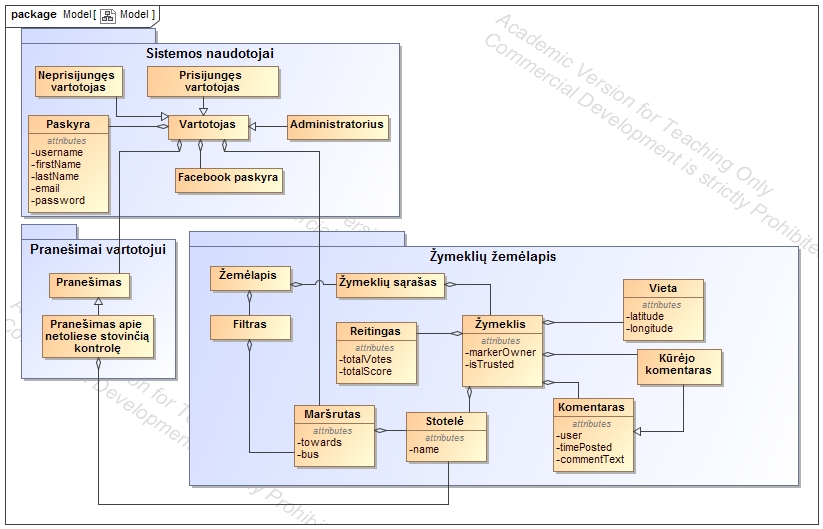
\includegraphics[scale=0.6]{img/esybiu_diagrama2}
				\caption{Esybių diagrama}
				\label{img:Esybių diagrama}
			\end{figure}
\subsection{Reikalavimų - esybių atsekamumo matrica}
Šiame skyriuje pateikiama reikalavimų - esybių atsekamumo matrica, kurioje galima matyti, kokios esybės naudojamos kiekviename reikalavime. (žr. \ref{img:Reikalavimų matrica} pav.).
	\begin{figure}[H]
				\centering
				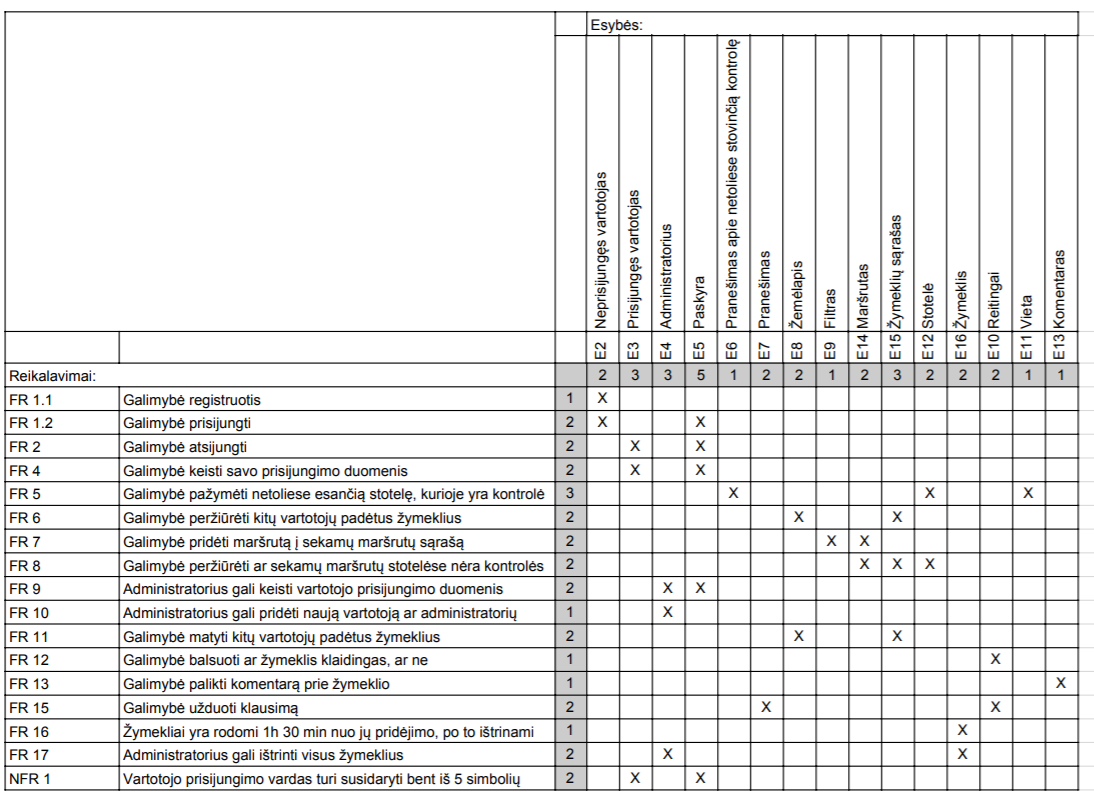
\includegraphics[scale=0.4]{img/esybiu_matrica}
				\caption{Reikalavimų atsekamumo matrica}
				\label{img:Reikalavimų matrica}
			\end{figure}

\subsection{Žodynas}
Pateikiamos sistemoje naudojamos esybės, taip pat - jų trumpi aprašymai.
				\begin{enumerate}[label=E\arabic*,itemsep=-2mm]
					\item \textit{Vartotojas} - klientas, prisiregistravęs prie aplikacijos.
					\item \textit{Neprisijungęs vartotojas} - vartotojas, kuris nėra atlikęs prisijungimo procedūros programėlėje ir neturi galiojančios prisijungimo sesijos.
					\item \textit{Prisijungęs vartotojas} - vartotojas, sėkmingai atlikęs prisijungimo procedūrą programėlėje ir turintis galiojančią prisijungimo sesiją.
					\item \textit{Administratorius} - vartotojas, atsakingas už sklandų programėlės veikimą, turintis padidintas teises paprastų vartotojų atžvilgiu.
					\item \textit{Paskyra} - registracijos metu kliento nurodyti duomenys (vardas, pavardė, elektroninio pašto adresas, prisijungimo vardas, slaptažodis), padedantys identifikuoti klientą.
					\item \textit{Facebook paskyra} - registracijos metu kliento autentifikacijai naudota paskyra.
					\item \textit{Pranešimas} - sistemos informacinė žinutė vartotojui naudojant Android pranešimus (angl. push notifications).
					\item \textit{Žemėlapis} - virtualus žemėlapis, kuriame matomi visi vartotojų pažymėti aktyvūs žymekliai, atitinkantys vartotojo nustatytą paieškos filtrą.
					\item \textit{Filtras} - savybė, pagal kurią filtruojama, kurių stotelių žymeklius vartotojui rodyti žemėlapyje.
					\item \textit{Reitingas} - žymeklio patikimumo rodiklis, žymintis pagal vartotojų balsus nustatomą tikimybę, kad žymeklio vietoje stovi keleivių kontrolė. 
					\item \textit{Vieta} - GPS prieigos pagalba tiksliai nustatytos objekto buvimo koordinatės.
					\item \textit{Stotelė} - vieta, pro kurią reguliariai kursuoja viešasis transportas.
					\item \textit{Komentaras} - vartotojo nurodyta papildoma informacija apie žymeklio vietoje stovinčią keleivių kontrolę.
					\item \textit{Maršrutas} - tam tikro autobuso kelionės metu aplankomų stotelių sąrašas.
					\item \textit{Keleivių kontrolė} - kontrolieriai, tikrinantys, ar keleiviai turi galiojančius ir tinkamos nuolaidų grupės bilietus
					\item \textit{Programėlė} - aplikacija, kurioje vartotojas gali pamatyti ar pažymėti žemėlapių vietas, kuriose yra keleivių kontrolė.
					\item \textit{Facebook} - socialinis tinklas “Facebook”.
				\end{enumerate}
\subsection{Vartotojo Sąsajos Langai}
Išvardinti visi esminiai sistemos grafinės sąsajos elementai
				\begin{enumerate}[label=VSL\arabic*,itemsep=-2mm]
					\item \textit{Prisijungimo langas} - programėlės langas, į kurį patenka naujas vartotojas, ją parsisiuntęs. Šiame lange taip pat yra nuoroda į registracijos langą ir prisijungimą per Facebook API.
					\item \textit{Registracijos langas} - programėlės langas, kuriame vartotojas suveda savo registracijos duomenis: vardą, pavardę, prisijungimo vardą, slaptažodį, el. paštą ir užbaigia registraciją.
					\item \textit{Pagrindinis langas} - tai pradinis langas, į kurį patenka prisijungęs vartotojas. Šiame lange matomas žemėlapis, GPS įrenginio pagalba jame sucentruota vartotojo buvimo vieta ir tame regione esantys žymekliai, jei jų yra.
					\item \textit{Profilio redagavimo langas} - tai langas, kuriame vartotojas gali pakeisti asmeninius duomenis, tokius kaip: vartotojo vardą, vardą ir pavardę, slaptažodį, el. paštą.
					\item \textit{Žymeklio informacinis langas} - langas, kuriame vartotojas mato visą informaciją apie pasirinktą konkretų žymeklį: žymeklį padėjusio vartotojo komentaras, kitų vartotojų komentarai, žemėlapio vieta, kurioje padėtas žymeklis. Taip pat vartotojas šiame lange gali palikti savo komentarą, balsuoti dėl žymeklio teisingumo. 
					\item \textit{“My favourite routes” langas} - tai vartotojo sekamų miesto autobusų maršrutų sąrašo langas, kuriame jis gali įtraukti iš sąrašo naujus sekamus maršrutus.
					\item \textit{Stotelių paieškos langas} - tai langas, į kurį vartotojas patenka Pagrindiniame lange paspaudęs mygtuką “Place marker”. Šiame lange vartotojas gali pasirinkti stotelę iš sąrašo.
					\item \textit{Žymeklio pridėjimo langas} -  tai langas, kuriame vartotojas, įvedęs komentarą apie žymeklį, jį prideda į sistemą.
					\item \textit{D.U.K. langas} - tai langas, į kurį varototjas patenka paspaudęs informacinę ikoną Pagrindiniame lange. Šiame lange yra surašyti visi dažniausiai užduodami klausimai ir atsakymai į juos.
					\item \textit{Klausimo uždavimo langas} - tai langas, į kurį vartotojas patenka iš D.U.K. lango ir kuriame įvedus klausimą į formą ir el. pašto adresą, galima išsiųsti klausimą administracijai.
				\end{enumerate}
\subsection{Užduotys}

Šiame skyriuje grafine diagrama pateikiamos užduotys, kurias gali atlikti vartotojai ir administratoriai (žr. \ref{img:uzduotys} pav.).
	\begin{figure}[H]
				\centering
				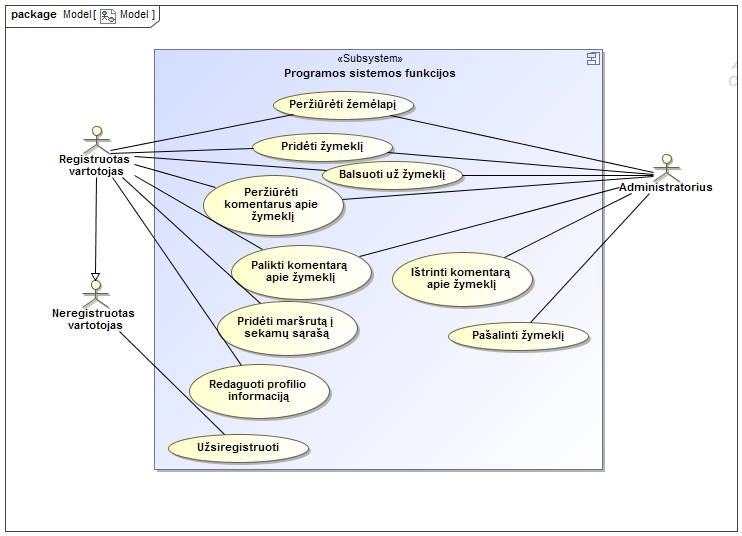
\includegraphics[scale=0.5]{img/uzduotys}
				\caption{Užduotys}
				\label{img:uzduotys}
			\end{figure}

\subsection{Užduočių aprašai}
\label{sec:Užduočių aprašai}
Skyriuje \ref{sec:Užduočių aprašai} pateikti užduočių aprašai kartu su pagrindiniais, alternatyviais scenarijais ir šabloniniais grafikos elementais.
\subsubsection{UC1 Registracija}
	Šiame skyriuje aprašomas vartotojo registracijos procesas,  kuris yra detaliai išnagrinėtas sekų diagramoje (žr. \ref{img:Registracijos sekų diagrama} pav.). 
	Procesą iliustruoja registracijos lango maketas (žr. \ref{img:registracija} pav.).

	\textbf{Pagrindinis scenarijus:}\\
	Vartotojas įsijungia programėlę ir patenka į prisijungimo langą. Joje spaudžia mygtuką “Register” ir patenka į registracijos langą. 
	Registracijos lange vartotojas įveda prisijungimo vardą, savo vardą, pavardę, el. paštą, slaptažodį, slaptažodį pakartoja bei paspaudžia 
	“Create my account”. Anketa sėkmingai sukuriama, vartojo įvesti duomenys išsaugomi duomenų bazėje ir vartotojas perkeliamas į prisijungimo langą.

	\textbf{Alternatyvūs scenarijai:}
	\begin{enumerate}[itemsep=-2mm]
		\item Jei vartotojo įvestame prisijungimo varde nėra 5 simbolių, programa pateikia informacinį pranešimą, kad prisijungimo vardas netinkamas, nes jame turi būti bent 5 simboliai.
		\item Jei vartotojo įvestas prisijungimo vardas duomenų bazėje jau egzistuoja, tada vartotojui programa pateikia informacinį pranešimą, kad prisijungimo vardas netinkamas, nes jau yra vartotojas su tokiu prisijungimo vardu.
		\item Jei vartotojo įvestas prisijungimo vardas yra per ilgas, tada vartotojui programa pateikia informacinį pranešimą, kad prisijungimo vardas netinkamas, nes prisijungimo vardas negali būti ilgesnis nei 15 simbolių eilutė.
		\item Jei įvestame varde ar pavardėje yra skaičių, programa pranešą, kad vardas arba pavardė yra nevalidūs.
		\item Jei vartotojo įvestas el. paštas neatitinka el. pašto formato, programa informuoja vartotoją, kad įvestas el. paštas netinkamas.
		\item Jei įvestame slaptažodyje nėra skaičiaus ar didžiosios raidės, arba jis yra trumpesnis nei 5 simboliai, tada vartotojui programa pateikia informacinį pranešimą, kad slaptažodis netinkamas, jame privalo būti didžioji raidė ir skaičius ir kad jį turi sudaryti bent 5 simboliai. Jei  vartotojo įvestas slaptažodis yra per ilgas, tada vartotojui programa pateikia informacinį pranešimą, kad slaptažodis netinkamas, nes slaptažodis negali būti ilgesnis nei 20 simbolių eilutė.
		\item Jei slaptažodžio bei slaptažodžio pakartojimo laukai nesutampa, tada vartotojui programa pateikia informacinį pranešimą, kad įvesti slaptažodžiai nesutampa.
		\item Jei dėl trikdžių duomenų bazėje vartotojui prisiregistruoti nepavyksta, tada vartotojui programa pateikia informacinį pranešimą, kad sistemoje įvyko klaida ir siūloma pabandyti prisiregistruoti vėliau.
	\end{enumerate} 
	    \begin{figure}[H]
				\centering
				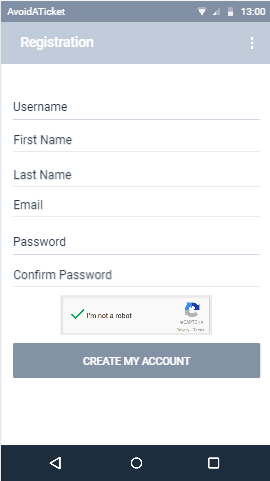
\includegraphics[scale=0.55]{img/mockup_registration}
				\caption{Registracijos lango maketas}
				\label{img:registracija}
			\end{figure}
		\begin{figure}[H]
				\centering
				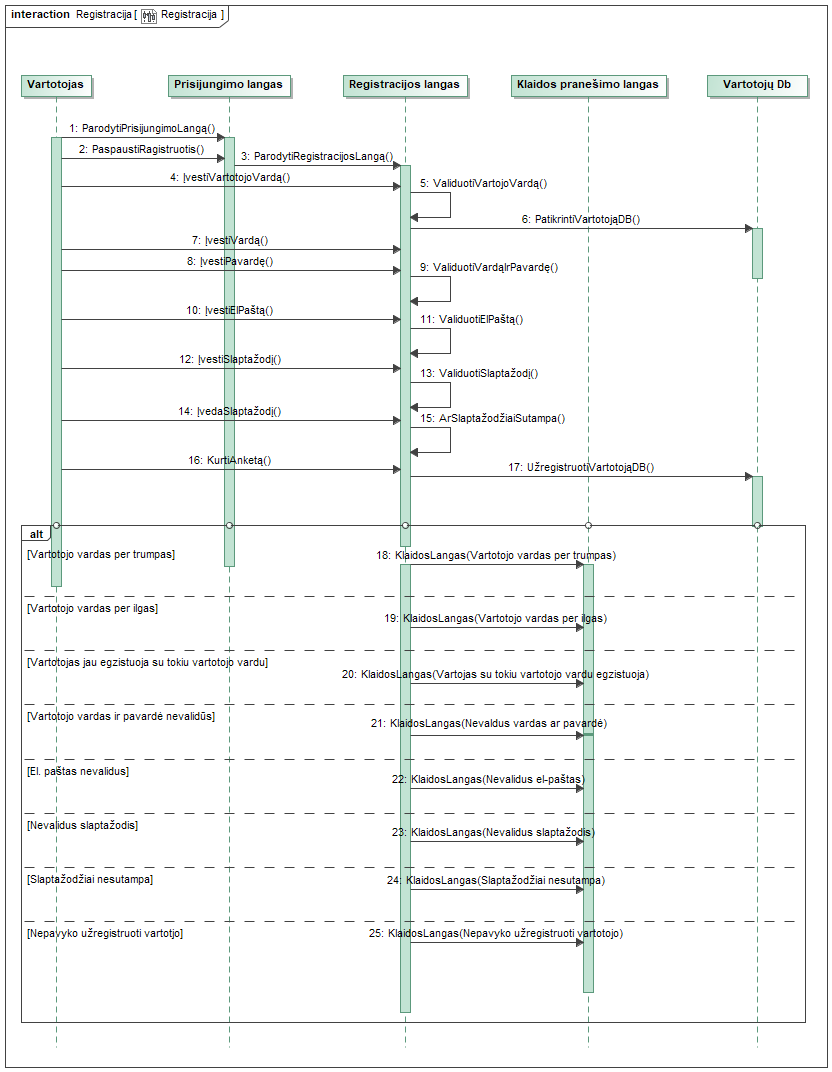
\includegraphics[scale=0.55]{img/RegistracijaSequence}
				\caption{Registracijos sekų diagrama}
				\label{img:Registracijos sekų diagrama}
			\end{figure}

\subsubsection{UC2 Prisijungimas}
	Šiame skyriuje aprašomas vartotojo prisijungimo prie aplikacijos procesas,  kuris yra detaliai išnagrinėtas sekų diagramoje (žr. \ref{img:Prisijungimo sekų diagrama} pav.). 
	Procesą iliustruoja prisijungimo lango maketas (žr. \ref{img:prisijungimas} pav.).

	\textbf{Pagrindinis scenarijus:}\\
	Vartotojas įsijungia programėlę ir patenka į prisijungimo langą. Prisijungimo lange įveda savo prisijungimo vardą ir slaptažodį, 
	spaudžia mygtuką “Login”, prisijungia ir yra perkeliamas į pagrindinį langą.
	
	\textbf{Alternatyvūs scenarijai:}
	\begin{enumerate}[itemsep=-2mm]
		\item Jei vartotojas praeitą sesiją neatsijungė, tada programėlė automatiškai prijungia vartotoją prie programėlės ir iškart vartotoją perkelia į pagrindinį langą.
		\item Jei vartotojas su tokiu prisijungimo vardu duomenų bazėje nebuvo rastas, tada vartotojui programa pateikia informacinį pranešimą, kad vartotojas su tokiu prisijungimo vardu programėlėje neegzistuoja.
		\item Jei vartotojo įvestas slaptažodis šiam prisijungimo vardui nesutampa su slaptažodžiu, esančiu sistemoje, tada vartotojui programa pateikia informacinį pranešimą, kad įvestas slaptažodis yra neteisingas.
		\item Jei vartotojas prisijungimo lange spaudžia “Continue with Facebook” ir vartotojo “Facebook” programėlės anketa sėkmingai panaudojama prisijungimui prie “AvoidATicket” programėlės, tada vartotojas yra prijungiamas ir perkeliamas į pagrindinį langą.
		\item Jei vartotojas prisijungimo lange spaudžia “Continue with Facebook” ir vartotojo “Facebook” programėlės anketos nepavyksta panaudoti prisijungimui prie “AvoidATicket” programėlės, tada vartotojui programa pateikia informacinį pranešimą, kad “Facebook” aplikacijos prisijungimo duomenų panaudoti nepavyko.
		\item Jei dėl trikdžių duomenų bazėje vartotojui prisijungti nepavyksta, tada vartotojui programa pateikia informacinį pranešimą, kad sistemoje įvyko klaida ir siūloma pabandyti prisijungti vėliau.
	\end{enumerate} 
	\begin{figure}[H]
				\centering
				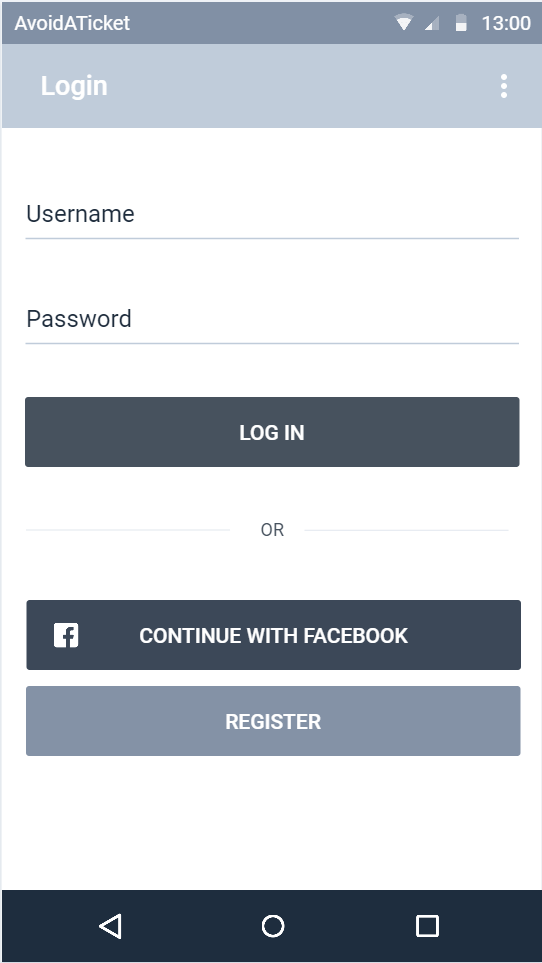
\includegraphics[scale=0.3]{img/mockup_login}
				\caption{Prisijungimo lango maketas}
				\label{img:prisijungimas}
			\end{figure}

	\begin{figure}[H]
				\centering
				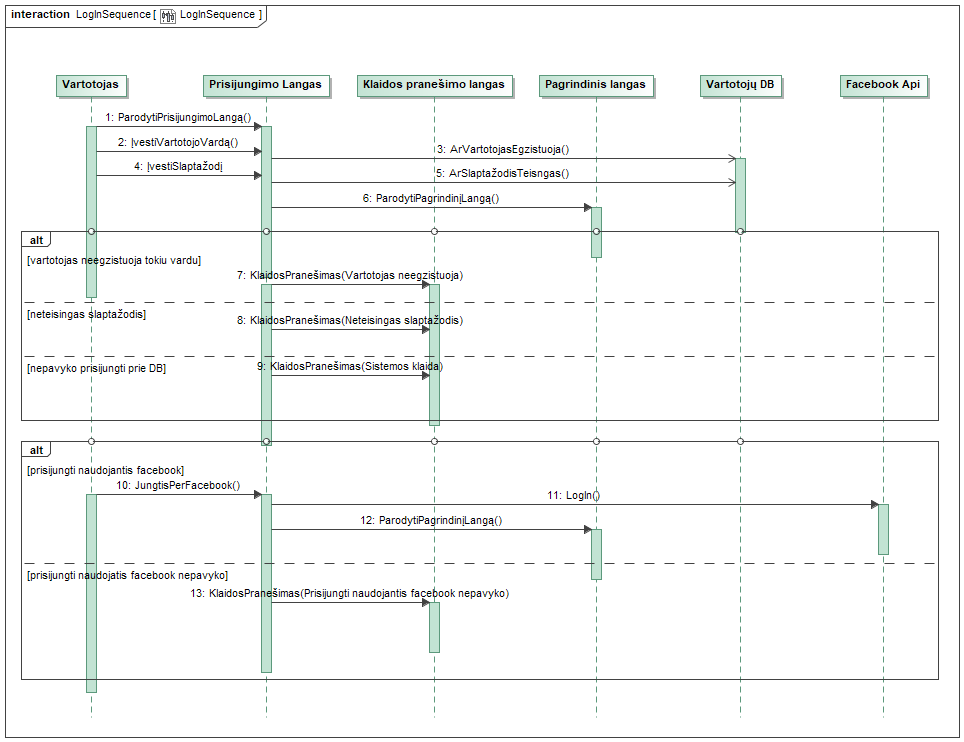
\includegraphics[scale=0.5]{img/LogInSequence}
				\caption{Prisijungimo sekų diagrama}
				\label{img:Prisijungimo sekų diagrama}
			\end{figure}

\subsubsection{UC3 Profilio duomenų redagavimas}
	Šiame skyriuje aprašomas vartotojo profilio duomenų redagavimo procesas,  kuris yra detaliai išnagrinėtas sekų diagramoje (žr. \ref{img:profilio redagavimas RD} pav.). 
	Procesą iliustruoja profilio duomenų redagavimo lango maketas (žr. \ref{img:profilio redagavimas} pav.).

	\textbf{Pagrindinis scenarijus:}\\
	Vartotojas pagrindiniame lange spaudžia mygtuką, ant kurio parašytas jo vardas ir pavardė, ir tada patenka į profilio redagavimo langą. Ten iš el. pašto, slaptažodžio, vardo, pavardės laukų paspaudžia ant norimos pakeisti reikšmės lauko ir įveda naują reikšmę.Tada paspaudžia mygtuką “Save” ir pakeisti duomenys sistemos išsaugomi duomenų bazėje. Vartotojas apie tai informuojamas informaciniu pranešimu. Pakeitęs duomenis, vartotojas paspaudžia mygtuką “Back” ir grįžtą į pagrindinį langą.

	\textbf{Alternatyvūs scenarijai:}
	\begin{enumerate}[itemsep=-2mm]
		\item Jei įvestame slaptažodyje nėra skaičiaus ar didžiosios raidės, arba jis yra trumpesnis nei 5 simboliai, tada vartotojui programa pateikia informacinį pranešimą, kad slaptažodis netinkamas, jame privalo būti didžioji raidė ir skaičius ir kad jį turi sudaryti bent 5 simboliai.
		\item Jei vartotojo įvestas prisijungimo vardas duomenų bazėje jau egzistuoja, tada vartotojui programa pateikia informacinį pranešimą, kad prisijungimo vardas netinkamas, nes jau yra vartotojas su tokiu prisijungimo vardu.
		\item Jei vartotojo įvestame prisijungimo varde nėra 5 simbolių arba yra specialiųjų simbolių, programa pateikia informacinį pranešimą, kad prisijungimo vardas netinkamas, nes jame turi būti bent 5 simboliai ir jame negali būti jokių specialiųjų simbolių.
		\item Jei vartotojo įvestas el. paštas neatitinka el. pašto formato, programa informuoja vartotoją, kad įvestas el. paštas netinkamas.
		\item Jei vartotojo įvestas prisijungimo vardas yra per ilgas, tada vartotojui programa pateikia informacinį pranešimą, kad prisijungimo vardas netinkamas, nes prisijungimo vardas negali būti ilgesnis nei 15 simbolių eilutė.
		\item Jei  vartotojo įvestas slaptažodis yra per ilgas, tada vartotojui programa pateikia informacinį pranešimą, kad slaptažodis netinkamas, nes slaptažodis negali būti ilgesnis nei 20 simbolių eilutė.
		\item Jei dėl trikdžių duomenų bazėje vartotojui pakeisti duomenų nepavyksta, tada vartotojui programa pateikia informacinį pranešimą, kad sistemoje įvyko klaida ir siūloma pabandyti prisiregistruoti vėliau.
		\item Vartotojas keičia slaptažodžio lauką, po pakeitimo slaptažodžio lauko ir slaptažodžio patvirtinimo lauko reikšmės nesutampa, jis spaudžia “Save” mygtuką, sistema atvaizduoja informacinį pranešimą, jog slaptažodžiai nesutampa, dėl to pakeitimai neįvykdyti.
	\end{enumerate} 
	\begin{figure}[H]
				\centering
				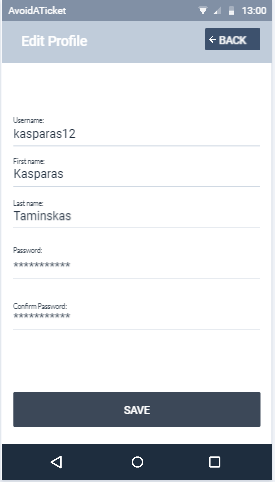
\includegraphics[scale=0.55]{img/mockup_profileedit}
				\caption{Profilio redagavimas}
				\label{img:profilio redagavimas}
			\end{figure}
		\begin{figure}[H]
				\centering
				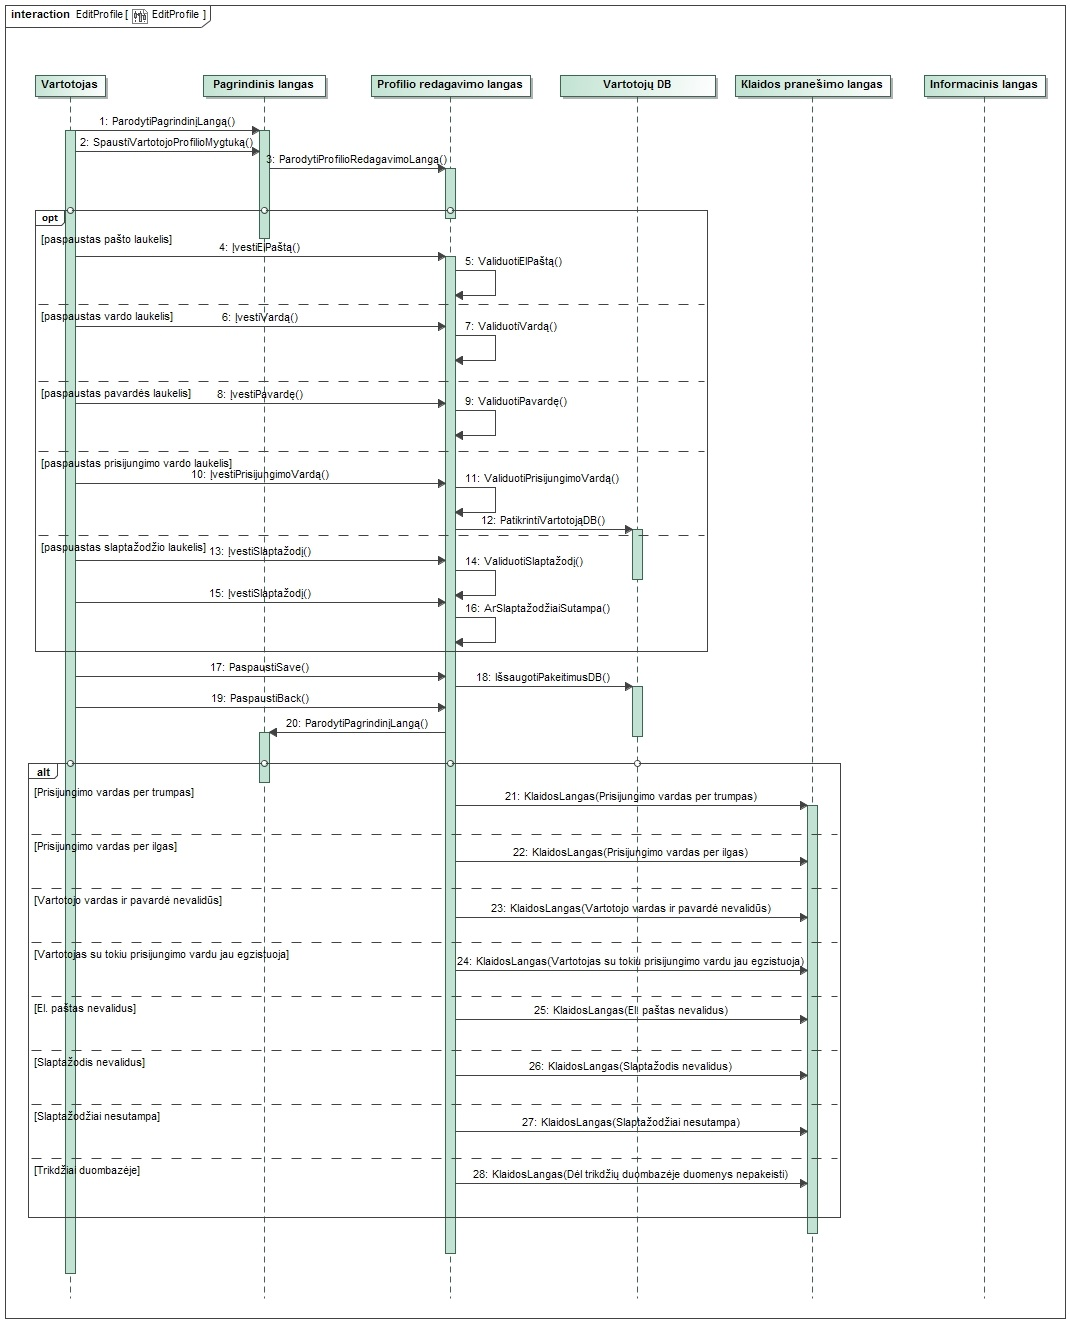
\includegraphics[scale=0.4]{img/EditProfileSequence}
				\caption{Profilio redagavimo sekų diagrama}
				\label{img:profilio redagavimas RD}
			\end{figure}

\subsubsection{UC4 Komentaro apie žymeklį pridėjimas}
	Šiame skyriuje aprašomas komentaro apie žymeklį pridėjimo procesas,  kuris yra detaliai išnagrinėtas sekų diagramoje (žr. \ref{img:Žymeklio informacijos langas RD} pav.). 
	Procesą iliustruoja komentaro apie žymeklį pridėjimo lango maketas (žr. \ref{img:Žymeklio informacijos langas1} pav.).

	\textbf{Pagrindinis scenarijus:}\\
    Vartotojas paspaudžia ant žymeklio, sistema jį nukelia į žymeklio informacijos langą. Vartotojas žymeklio informacijos lange įrašo komentarą į tam skirtą laukelį, spaudžia “Add Comment”. Sistema įrašo komentarą apie žymeklį į duomenų bazę. Sistema atvaizduoja komentarą komentarų sąrašo viršuje. Šiame lange vartotojas taip pat balsuoja: suteikia arba numuša reitinga žymekliui.

	\textbf{Alternatyvūs scenarijai:}
	\begin{enumerate}[itemsep=-2mm]
		\item Jei dėl trikdžių bandant pasiekti internetą, nepavyksta į duomenų bazę įrašyti vartotojo komentaro, tada vartotojui programa pateikia informacinį pranešimą, kad sistemoje įvyko klaida ir siūloma pabandyti vėliau.
		\item Vartotojas neįrašo jokio teksto į tam skirtą komentavimo laukelį ir spaudžia “Add Comment”, sistema išmeta informacinį pranešimą, jog komentaro palikti nepavyko, nes komentaro laukas tuščias.
	\end{enumerate} 
		\begin{figure}[H]
				\centering
				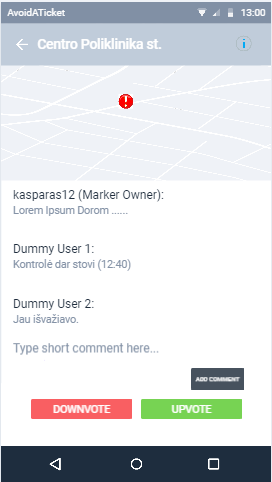
\includegraphics[scale=0.6]{img/mockup_markerInfoWindow}
				\caption{Žymeklio informacijos langas}
				\label{img:Žymeklio informacijos langas1}
			\end{figure} 
		\begin{figure}[H]
				\centering
				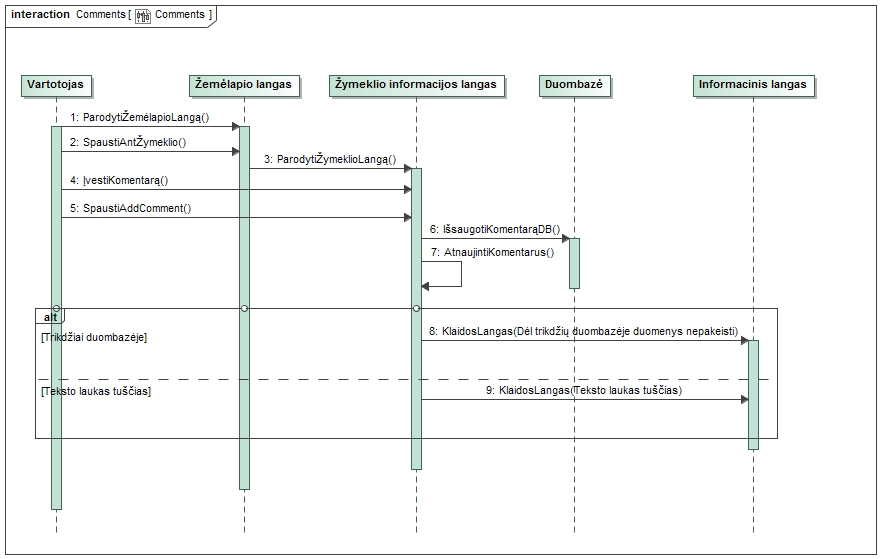
\includegraphics[scale=0.5]{img/CommentsSequence}
				\caption{Žymeklio informacijos lango sekų diagrama}
				\label{img:Žymeklio informacijos langas RD}
			\end{figure}

\subsubsection{UC5 Maršruto pridėjimas į sekamų sąrašą}
	Šiame skyriuje aprašomas maršruto pridėjimo į sekamų sąrašą procesas,  kuris yra detaliai išnagrinėtas sekų diagramoje (žr. \ref{img:Maršruto pridėjimo langas RD} pav.). 
	Procesą iliustruoja maršruto pridėjimo į sekamų sąrašą lango maketas (žr. \ref{img:Maršruto pridėjimo langas} pav.).
	
	\textbf{Pagrindinis scenarijus:}\\
	Vartotojas lange “Mano maršrutai” spaudžia “+” ir sistema atidaro bendrą miesto autobusų sąrašą, kuriame neįtraukti 
	vartotojo jau anksčiau pažymėti autobusai, kurių maršrutai įtraukti į sekamų sąrašą. Vartotojas paspaudžia ant jį 
	dominančio autobuso sąrašo elemento iš bendro miesto autobusų sąrašo, tada sistema įtraukia pasirinktą autobuso maršrutą 
	į vartotojo sekamų maršrutų sąrašą. Sistema parodo pranešimą pranešimų srityje “Autobuso {autobusas} maršrutas sėkmingai 
	įtrauktas į sekamų maršrutų sąrašą“. Sistema perkelia vartotoją i “Mano maršrutai” langą. Vartotojo pasirinktas autobuso 
	elementas atvaizduojamas “Mano maršrutai” lango sąrašo gale.

	\textbf{Alternatyvūs scenarijai:}
	\begin{enumerate}[itemsep=-2mm]
		\item Jei dėl trikdžių bandant pasiekti internetą, nepavyksta vartotojui parodyti bendrą autobusų sąrašą ar pridėti autobuso maršrutą į sekamų maršrutų sąrašą, tada vartotojui programa pateikia informacinį pranešimą, kad sistemoje įvyko klaida ir siūloma pabandyti vėliau.
	\end{enumerate} 
		\begin{figure}[H]
				\centering
				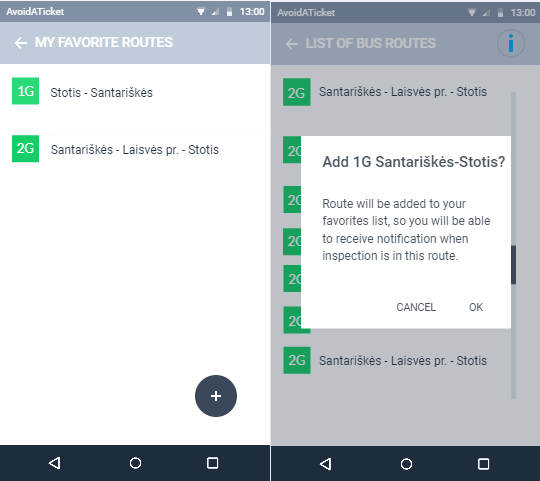
\includegraphics[scale=1.5]{img/mockup_AddRoute}
				\caption{Maršruto pridėjimo langas}
				\label{img:Maršruto pridėjimo langas}
			\end{figure}
		\begin{figure}[H]
				\centering
				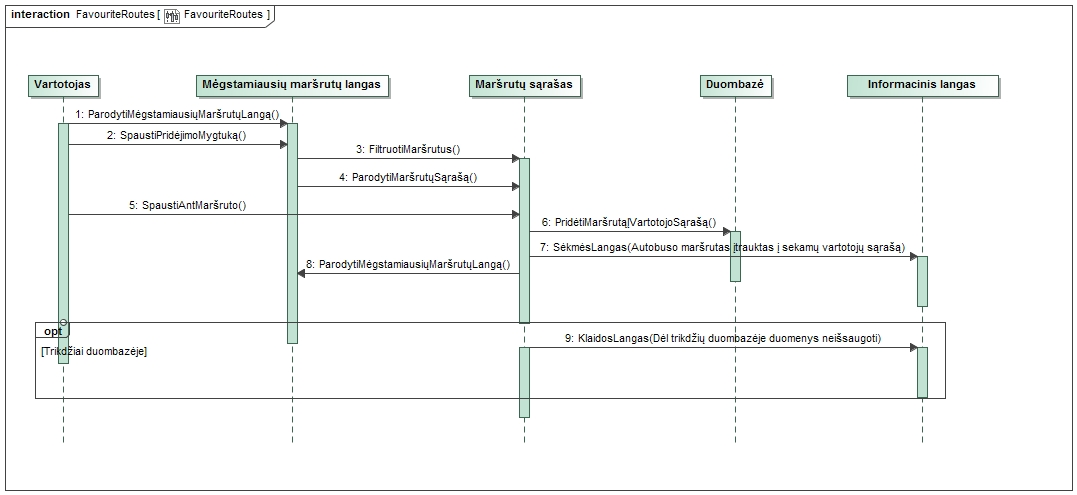
\includegraphics[scale=0.45]{img/FavouriteRoutesSequence}
				\caption{Maršruto pridėjimo lango sekų diagrama}
				\label{img:Maršruto pridėjimo langas RD}
			\end{figure}

\subsubsection{UC6 Atsijungimas}
	Šiame skyriuje aprašomas vartotojo atsijungimo nuo aplikacijos procesas,  kuris yra detaliai išnagrinėtas sekų diagramoje (žr. \ref{img:Atsijungimo sekų diagrama} pav.).
	
	\textbf{Pagrindinis scenarijus:}
	Vartotojas pagrindiniame lange paspaudžia “Log Off”, sistema jį atjungia ir vartotojas yra nukeliamas į prisijungimo langą.
		\begin{figure}[H]
				\centering
				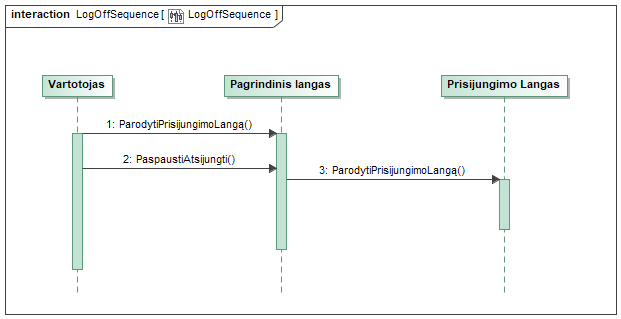
\includegraphics[scale=0.6]{img/LogOffSequence}
				\caption{Atsijungimo sekų diagrama}
				\label{img:Atsijungimo sekų diagrama}
			\end{figure}

\subsubsection{UC7 Žemėlapio ir jame esančių žymeklių peržiūra}
	Šiame skyriuje aprašomas žymeklių peržiūros procesas,  kuris yra detaliai išnagrinėtas sekų diagramoje (žr. \ref{img:Žemėlapio redagavimas. Žymeklių peržiūra} pav.). 
	Procesą iliustruoja žymeklių peržiūros lango maketas (žr. \ref{img:Pagrindinis langas} pav.).

	\textbf{Pagrindinis scenarijus:}\\
	Vartotojas prisijungęs prie programėlės patenka į pagrindinį langą, kuriame matomas žemėlapis ir visi galiojantys žymekliai (šauktuko metafora, žr. Sąsajos Lange). Paspaudęs ant žymeklio vartotojas mato stotelės pavadinimą, kurioje stovi kontrolė, taip pat kiek laiko praėjo nuo žymeklio padėjimo laiko. Programėlės pagrindinio lango apačioje vartotojas mato žymeklio reitingą.
	
	\textbf{Alternatyvūs scenarijai:}
	\begin{enumerate}[itemsep=-2mm]
		\item Jei vartotojas neturi davęs sutikimo programėlei naudotis GPS, tada ji prašo prieigos prie GPS pateikdama GPS prieigos dialogo langą. 
		\begin{enumerate}[itemsep=-2mm]
			\item Jei vartotojas paspaudžia “Accept”, programėlei duodamas sutikimas naudotis telefono GPS ir vartotojas yra nukeliamas į žemėlapio langą, kuriame rodomi visi galiojantys žymekliai.
			\item Jei vartotojas paspaudžia “Decline”, programa pateikia informacinį pranešimą, kad negali parodyti žemėlapio, nes vartotojas nesuteikė prieigos prie GPS. Vartotojas išjungia šį pranešimą ir programėlė išsijungia.
		\end{enumerate} 
		\item Jei programai nepavyksta rasti vartotojo buvimo vietos, tada vartotojui programa pateikia informacinį pranešimą, kad vartotojo buvimo vietos rasti nepavyko.
	\end{enumerate} 
		\begin{figure}[H]
				\centering
				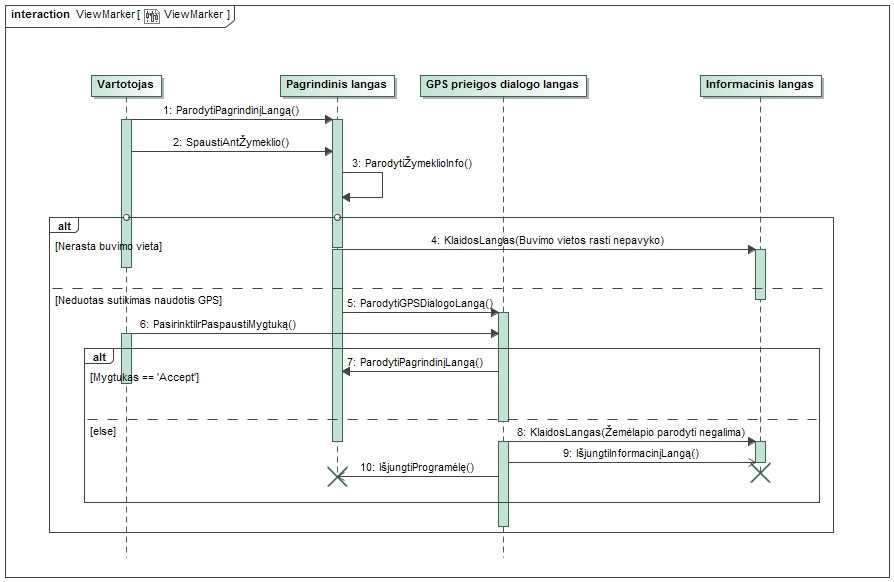
\includegraphics[scale=0.5]{img/ViewMarkerSequence}
				\caption{Žemėlapio peržiūros sekų diagrama}
				\label{img:Žemėlapio redagavimas. Žymeklių peržiūra}
			\end{figure}
	\begin{figure}[H]
				\centering
				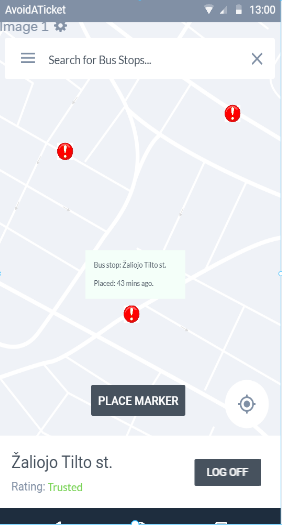
\includegraphics[scale=0.6]{img/mockup_Main_Window}
				\caption{Pagrindinis langas}
				\label{img:Pagrindinis langas}
			\end{figure}

\subsubsection{UC8 Žemėlapio redagavimas. Žymeklių pridėjimas}
	Šiame skyriuje aprašomas žymeklių pridėjimo procesas,  kuris yra detaliai išnagrinėtas sekų diagramoje (žr. \ref{img:Žymeklio pridėjimo langas RD} pav.). 
	Procesą iliustruoja žymeklių pridėjimo lango maketas (žr. \ref{img:Žymeklio pridėjimo langas RD} pav.).

	\textbf{Pagrindinis scenarijus:}\\
	Vartotojas pagrindiniame lange paspaudžia “Place Marker” ir yra nukeliamas į stotelių paieškos langą, kuriame matomas stotelių sąrašas. Vartotojas pasirenka stotelę iš sąrašo arba randa stotelę paieškos lauke įvedęs stotelės pavadinimo fragmentą ir yra nukeliamas į žymeklio pridėjimo langą, kuriame matomas žemėlapio fragmentas, stotelės pavadinimas, link kokios pusės važiuojant stovi kontrolė. Vartotojas palieka komentarą ir paspaudžia „Confirm”, tuomet sistema prideda žymeklį į atitinkamą vietą žemėlapyje.

	\textbf{Alternatyvūs scenarijai:}
	\begin{enumerate}[itemsep=-2mm]
		\item Jei vartotojas neturi davęs sutikimo programėlei naudotis GPS, tada ji prašo prieigos prie GPS pateikdama informacijos langą. 
		\begin{enumerate}[itemsep=-2mm]
			\item Jei vartotojas paspaudžia “Accept”, programėlei duodamas sutikimas naudotis telefono GPS ir vartotojas yra nukeliamas į žymeklių pridėjimo langą, kuriame rodomi visi galiojantys žymekliai.
			\item Jei vartotojas paspaudžia “Decline”, programa pateikia informacinį pranešimą, kad negali parodyti žemėlapio, nes vartotojas nesuteikė prieigos prie GPS.
		\end{enumerate} 
		\item Jei programai nepavyksta rasti vartotojo buvimo vietos, tada vartotojui programa pateikia informacinį pranešimą, kad vartotojo buvimo vietos rasti nepavyko.
		\item Jei vartotojas bando padėti žymeklį vietoje, kuri yra nutolusi daugiau nei 1.5 km nuo vartotojo, tada vartotojui programa pateikia informacinį pranešimą, kad vartotojas negali dėti žymeklių vietose, nutolusiose nuo vartotojo per daugiau nei 1.5 km.
	\end{enumerate} 
		\begin{figure}[H]
				\centering
				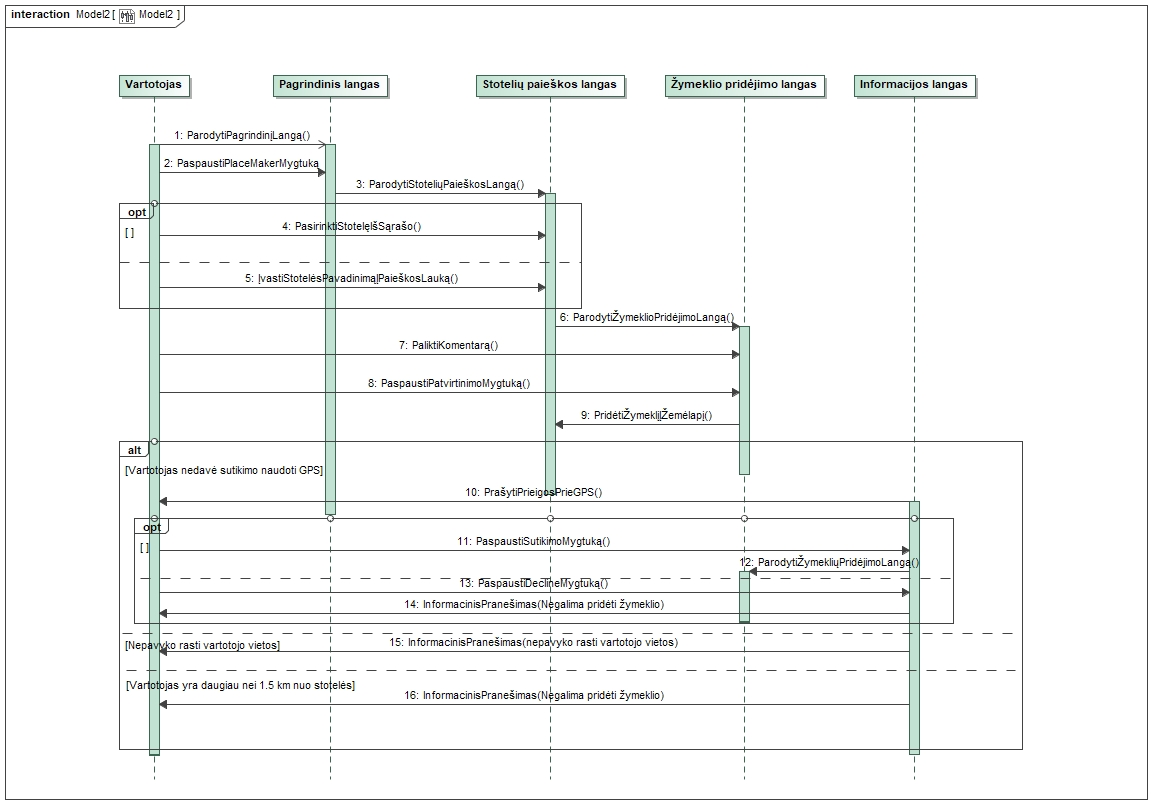
\includegraphics[scale=0.4]{img/AddMarkerSequence}
				\caption{Žymeklio pridėjimo sekų diagrama}
				\label{img:Žymeklio pridėjimo langas RD}
			\end{figure}
	\begin{figure}[H]
				\centering
				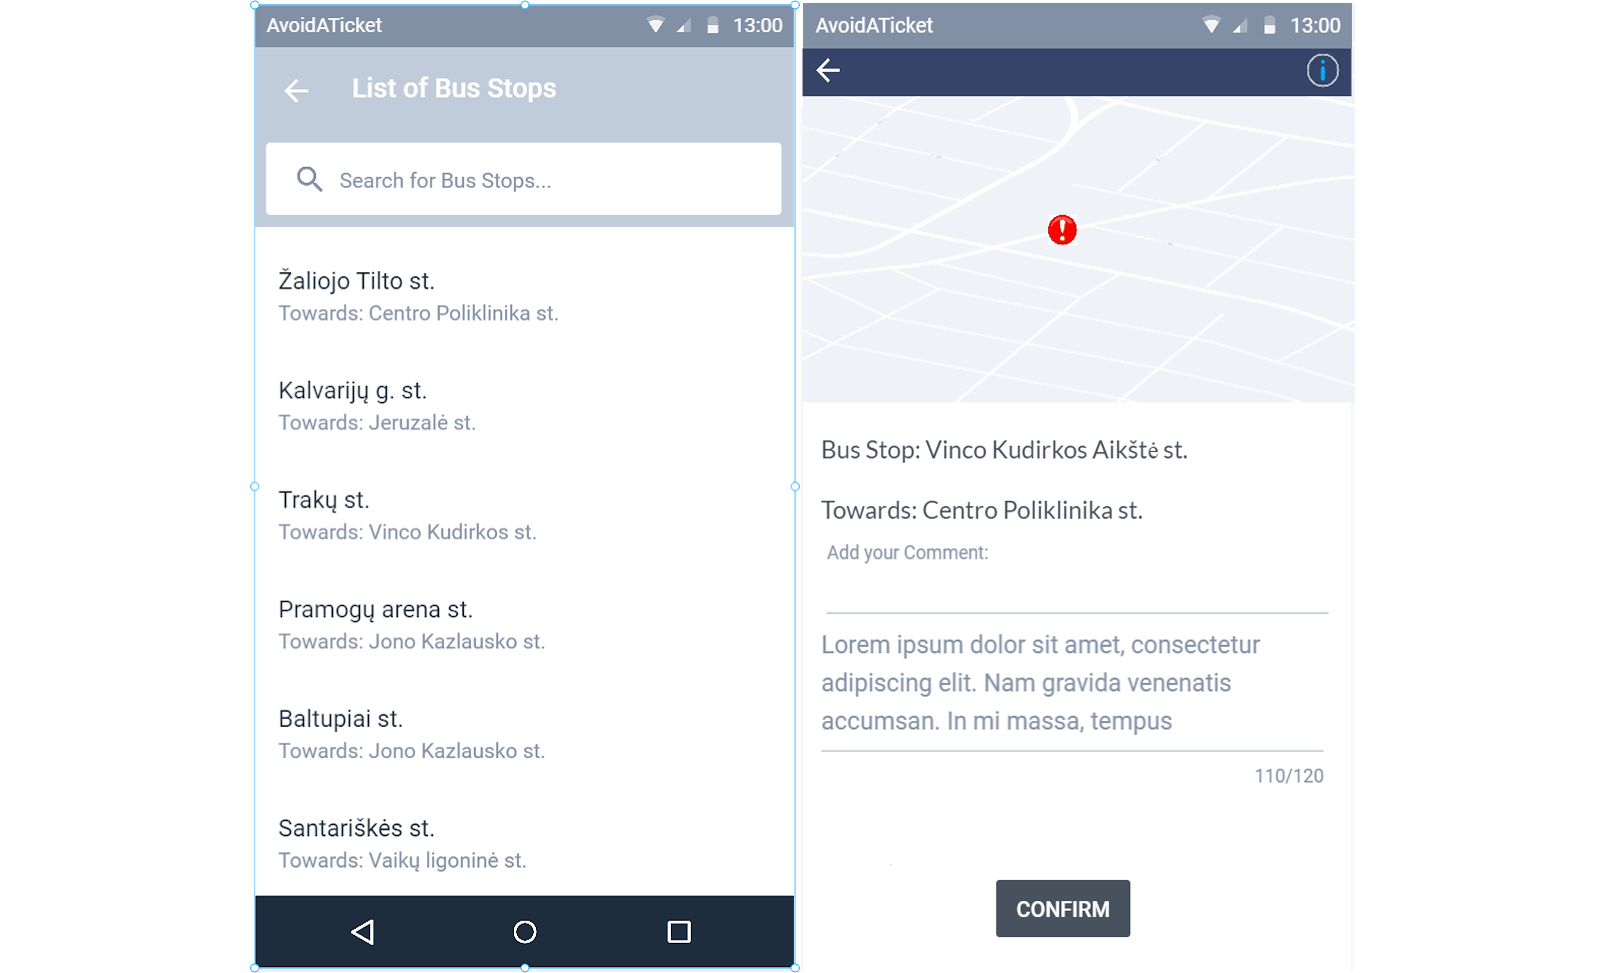
\includegraphics[scale=0.2]{img/mockup_AddMarker}
				\caption{Žymeklio pridėjimo langas}
				\label{img:Žymeklio pridėjimo langas}
			\end{figure}

\subsubsection{UC9 Žemėlapio redagavimas. Vartotojų balsavimas dėl žymeklio teisingumo}
	Šiame skyriuje aprašomas vartotojų balsavimo dėl žymeklio teisingumo procesas,  kuris yra detaliai išnagrinėtas sekų diagramoje (žr. \ref{img:Žymeklio informacijos RD} pav.). 
	Procesą iliustruoja balsavimo dėl žymeklio teisingumo lango maketas (žr. \ref{img:Žymeklio informacijos langas} pav.).

	\textbf{Pagrindinis scenarijus:}\\
	Vartotojas pagrindiniame lange paspaudžia ant pasirinkto galiojančio žymeklio, kuris yra ne toliau nei 1,5km nuo jo dabartinės padėties ir yra nukeliamas į žymeklio balsavimo langą. Jei kontrolė vartotojo pasirinkto žymeklio vietoje jau nebestovi, vartotojas paspaudžia mygtuką “Downvote”, sistema išsaugoja vartotojo balsą duomenų bazėje, žymintį, kad kontrolė pasitraukė iš pasirinkto žymeklio vietos. Jei kontrolė žymeklio vietoje vis dar stovi, vartotojas paspaudžia mygtuką “Upvote” ir sistema išsaugo vartotojo balsą duomenų bazėje, patvirtinantį, kad kontrolė dar yra pasirinkto žymeklio vietoje. Vartotojas, atidavęs savo balsą, yra perkeliamas į bendrą žemėlapio langą su visais galiojančiais žymekliais. Žymeklio, gavusio 51% balsų, žyminčių, kad kontrolė žymeklio vietoje jau nebestovi, pasitikėjimo reitingas yra pakeičiamas į „Not Trusted“.
	
	\textbf{Alternatyvūs scenarijai:}
	\begin{enumerate}[itemsep=-2mm]
		\item Jei vartotojas pasirenka žymeklį, esantį toliau nei 1,5km nuo jo esamos buvimo vietos, nustatytos pagal GPS, vartotojui nėra rodomas žymeklio balsavimo langas ir jam neleidžiama balsuoti.
		\item Jei programai nepavyksta rasti vartotojo buvimo vietos, tada vartotojui programa pateikia informacinį pranešimą, kad vartotojo buvimo vietos rasti nepavyko.
		\item Jei vartotojas bando balsuoti už tą patį žymeklį antrą kartą, sistema jam praneša, kad jis jau balsavo anksčiau ir neįskaito vartotojo balso.
	\end{enumerate} 
		\begin{figure}[H]
				\centering
				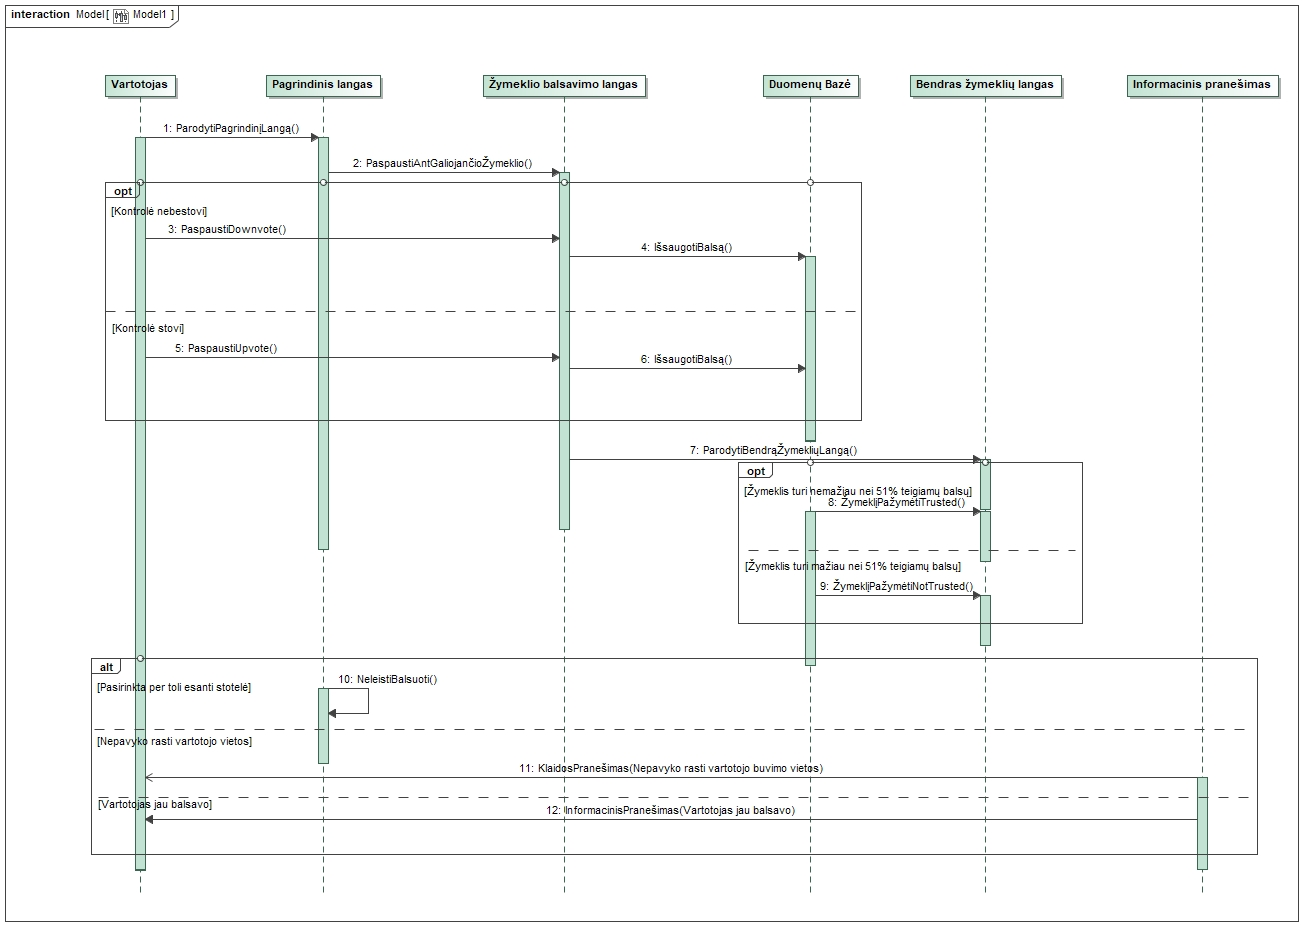
\includegraphics[scale=0.35]{img/VoteSequence}
				\caption{Žymeklio balsavimo sekų diagrama}
				\label{img:Žymeklio informacijos RD}
			\end{figure}
	\begin{figure}[H]
				\centering
				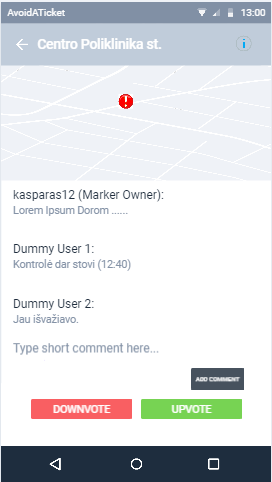
\includegraphics[scale=0.6]{img/mockup_markerInfoWindow}
				\caption{Žymeklio informacijos langas}
				\label{img:Žymeklio informacijos langas}
			\end{figure}

\subsubsection{UC10 Žemėlapio redagavimas. Administratoriaus žymeklių trynimas}
	Šiame skyriuje aprašomas žemėlapio radagavimo procesas,  kuris yra detaliai išnagrinėtas sekų diagramoje (žr. \ref{img:Žymeklio radagavimo langas} pav.).

	\textbf{Pagrindinis scenarijus:}\\
	Administratorius pagrindiniame lange paspaudžia “Clear Markers”, tada programėlė ištrina visus žymeklius, esamus žemėlapyje.

	\textbf{Alternatyvūs scenarijai:}
	\begin{enumerate}[itemsep=-2mm]
		\item Jei dėl trikdžių nepavykstą ištrinti bent vieno žymeklių, ištrinti žymekliai yra grąžinami į savo vietas ir programėlė informuoja administratorių informaciniu pranešimu, kad dėl trikdžių duomenų bazėje nepavyko ištrinti žymeklių ir siūloma administratoriui pabandyti vėliau.
		\item Administratorius pagrindiniame lange, žemėlapyje, pasirenka konkretų žymeklį, žemėlapio apačioje prie reitingo atsiranda mygtukas “Clear Marker”, administratorius jį paspaudžia ir ištrina tik tą vieną konkretų žymeklį.
	\end{enumerate} 
		\begin{figure}[H]
				\centering
				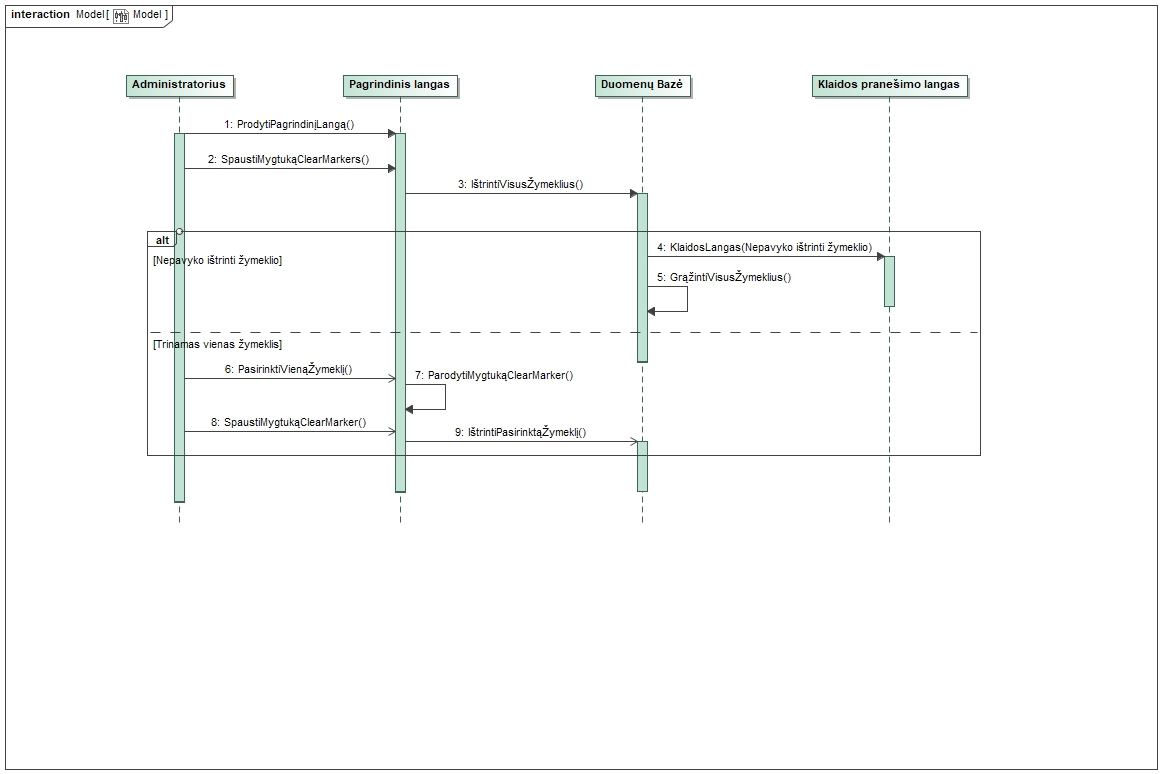
\includegraphics[scale=0.4]{img/AdminMarkerDeleteSequence}
				\caption{Žymeklio redagavimo robustiškumo diagrama}
				\label{img:Žymeklio radagavimo langas}
			\end{figure}


\subsubsection{UC11 Susisiekimas su administracija}
	Šiame skyriuje aprašomas susisiekimo su administracija procesas,  kuris yra detaliai išnagrinėtas sekų diagramoje (žr. \ref{img:Susisiekimas su administracija RD} pav.). 
	Procesą iliustruoja susisiekimo su administracija lango maketas (žr. \ref{img:Susisiekimas su administracija} pav.).

	\textbf{Pagrindinis scenarijus:}\\
	Vartotojas pagrindiniame lange paspaudžia “FAQ | Ask a question” ir patenka į D.U.K. langą. D.U.K lange vartotojas 
	spaudžia “Ask a question” mygtuką ir patenka į klausimo uždavimo langą. Klausimo uždavimo lange vartotojas įveda 
	savo el. paštą ir klausimą bei spaudžia “Send us the question”. Klausimas nusiunčiamas sėkmingai, o programa informuoja 
	vartotoją, kad klausimą nusiųsti pavyko.

	\textbf{Alternatyvūs scenarijai:}
	\begin{enumerate}[itemsep=-2mm]
		\item Jei vartotojas el. pašto lauką palieka tuščią, programa informuoja vartotoją, kad klausimo nusiųsti nepavyko, nes vartotojas nepateikė savo el. pašto.
		\item Jei vartotojo įvestas el. paštas neatitinka el. pašto formato, programa informuoja vartotoją, kad įvestas el. paštas netinkamas.
		\item Jei vartotojas klausimo lauką palieka tuščią, programa informuoja vartotoją, kad klausimo nusiųsti nepavyko, nes vartotojas klausimo lauką paliko tuščią.
	\end{enumerate} 
		\begin{figure}[H]
				\centering
				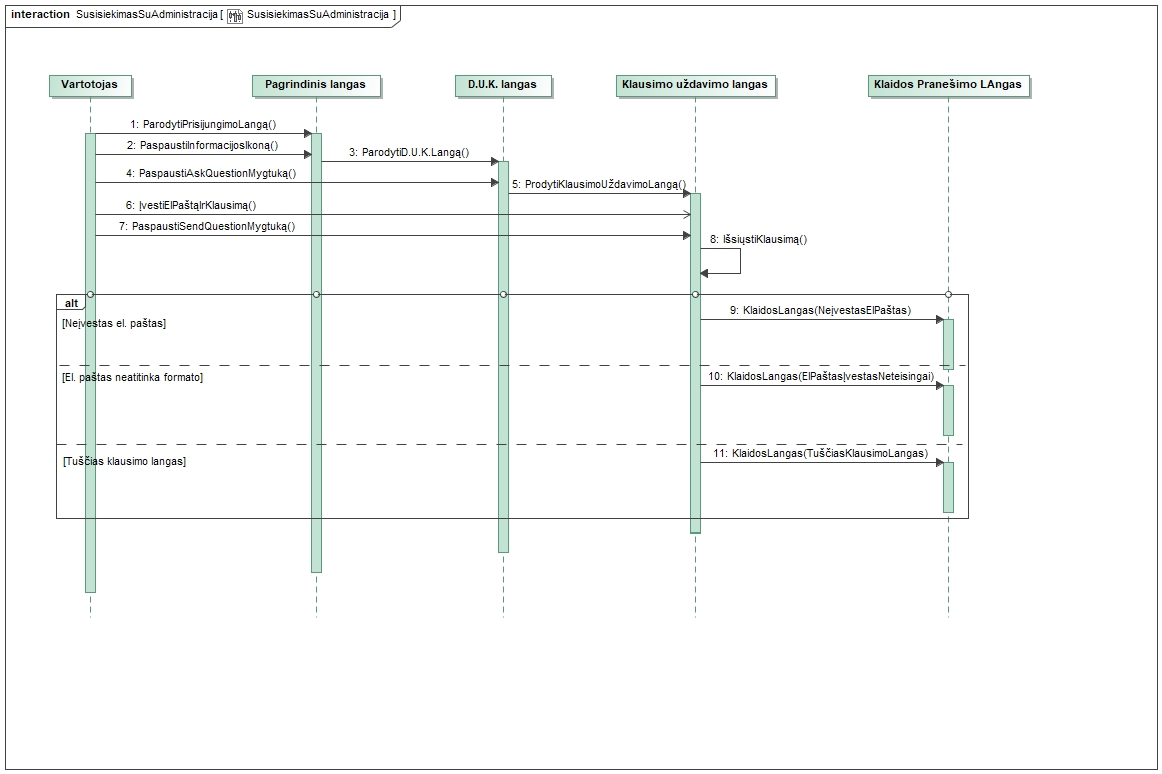
\includegraphics[scale=0.4]{img/ContactAdminSequence}
				\caption{Susisiekimo su administracija sekų diagrama}
				\label{img:Susisiekimas su administracija RD}
			\end{figure}
	\begin{figure}[H]
				\centering
				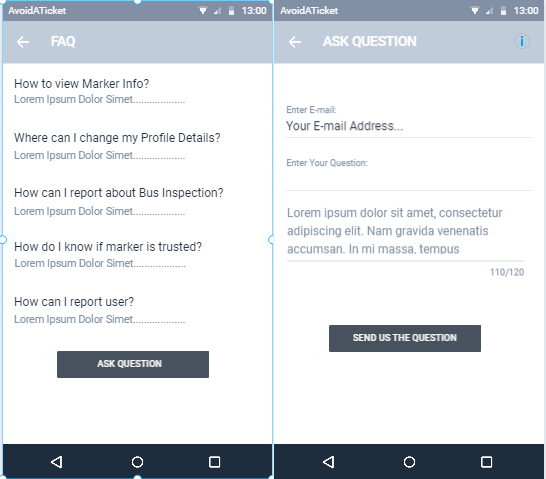
\includegraphics[scale=1.4]{img/mockup_admincomunication}
				\caption{Susisiekimas su administracija}
				\label{img:Susisiekimas su administracija}
			\end{figure}


\subsection{Reikalavimų - užduočių atsekamumo matrica}
Šiame skyriuje pateikiama reikalavimų - užduočių atsekamumo matrica, kurioje galima matyti, kaip užduotys susijusios su reikalavimais (žr. \ref{img:Užduočių matrica} pav.).
	\begin{figure}[H]
				\centering
				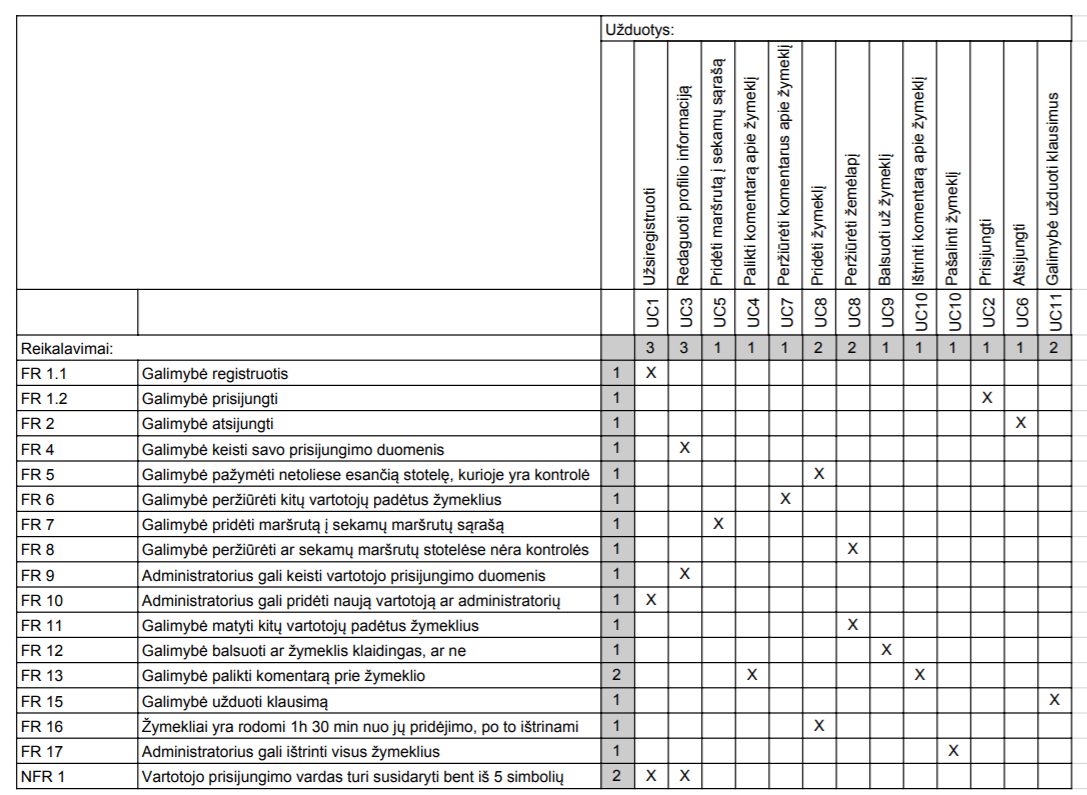
\includegraphics[scale=0.4]{img/uzduociu_matrica}
				\caption{Užduočių atsekamumo matrica}
				\label{img:Užduočių matrica}
			\end{figure}

\section{Testavimo planas}
	\subsection{TUC1 Registracijos testavimo scenarijus}
		\textbf{Testai}
		\begin{enumerate}[noitemsep,topsep=0pt]
			\item pagrindinis scenarijus
			\item registruotis, kai prisijungimo vardas sudarytas iš mažiau nei 5 simbolių arba iš daugiau nei 15 simbolių
			\item registruotis, kai įvestas jau užregistruotas prisijungimo vardas
			\item registruotis, kai varde/pavardėje yra skaičių
			\item registruotis, kai įvestas netinkamas el. pašto formatas
			\item registruotis, kai slaptažodyje nėra skaičiaus ar didžiosios raidės arba jis yra trumpesnis nei 5 simboliai ar ilgesnis nei 20 simbolių
			\item registruotis, kai įvesti slaptažodis ir pakartotinas slaptažodis skiriasi
		\end{enumerate}
		\textbf{}\\
		\textbf{Testas 1.1}\\
		\textbf{Tikslas:} ar veikia pagrindinis scenarijus\\
		\textbf{Prieš sąlygos:} programėlė įrašyta į įrenginį, vartotojas yra registracijos lange\\
		\textbf{Žingsniai:}
		\begin{enumerate}[noitemsep,topsep=0pt]
			\item Įvesti neužregistruotą prisijungimo vardą, savo vardą, pavardę, el. paštą, slaptažodį, pakartoti slaptažodį
			\item Paspausti mygtuką “Create my account” 
			\item Patikrinti, ar parodomas pranešimas apie sėkmingą registraciją sistemoje
		\end{enumerate}
		\textbf{}\\
		\textbf{Testas 1.2}\\
		\textbf{Tikslas:} ar sistema veikia korektiškai, kai įvestas prisijungimo vardas sudarytas iš mažiau nei 5 simbolių arba iš daugiau nei 15 simbolių\\
		\textbf{Prieš sąlygos:} programėlė įrašyta į įrenginį, vartotojas yra registracijos lange\\
		\textbf{Žingsniai:}
		\begin{enumerate}[noitemsep,topsep=0pt]
			\item Įvesti savo vardą, pavardę, el. paštą, slaptažodį, pakartoti slaptažodį
			\item Įvesti prisijungimo vardą, sudarytą iš mažiau nei 5 simbolių arba iš daugiau nei 15 simbolių
			\item Paspausti mygtuką “Create my account” 
			\item Patikrinti, ar prisijungimo vardo laukas nuspalvinamas raudonai ir ar atspausdinamas pranešimas, jog prisijungimo vardas turi būti sudarytas iš ne mažiau nei 5 simbolių, bet ne daugiau nei 15 simbolių
		\end{enumerate}
		\textbf{}\\
		\textbf{Testas 1.3}\\
		\textbf{Tikslas:} ar sistema veikia korektiškai, kai įvestas užregistruotas prisijungimo vardas\\
		\textbf{Prieš sąlygos:} programėlė įrašyta į įrenginį, vartotojas yra registracijos lange\\
		\textbf{Žingsniai:}
		\begin{enumerate}[noitemsep,topsep=0pt]
			\item Įvesti savo vardą, pavardę, el. paštą, slaptažodį, pakartoti slaptažodį
			\item Įvesti jau užregistruotą prisijungimo vardą
			\item Paspausti mygtuką “Create my account” 
			\item Patikrinti, ar prisijungimo vardo laukas nuspalvinamas raudonai ir ar atspausdinamas pranešimas, jog toks prisijungimo vardas jau yra naudojamas
		\end{enumerate}
		\textbf{}\\
		\textbf{Testas 1.4}\\
		\textbf{Tikslas:} ar sistema veikia korektiškai, kai įvestuose varde/pavardėje yra skaičių\\
		\textbf{Prieš sąlygos:} programėlė įrašyta į įrenginį, vartotojas yra registracijos lange\\
		\textbf{Žingsniai:}
		\begin{enumerate}[noitemsep,topsep=0pt]
			\item Įvesti neužregistruotą prisijungimo vardą, el. paštą, slaptažodį, pakartoti slaptažodį
			\item Įvesti savo vardą ir pavardę, iš kurių bent viename būtų skaičius
			\item Paspausti mygtuką “Create my account” 
			\item Patikrinti, ar atitinkamai vardo ir/ar pavardės laukas(-ai) nuspalvinamas raudonai ir ar atspausdinamas pranešimas, jog vardas ir pavardė negali turėti skaičių
		\end{enumerate}
		\textbf{}\\
		\textbf{Testas 1.5}\\
		\textbf{Tikslas:} ar sistema veikia korektiškai, kai įvestas netinkamas el. paštas\\
		\textbf{Prieš sąlygos:} programėlė įrašyta į įrenginį, vartotojas yra registracijos lange\\
		\textbf{Žingsniai:}
		\begin{enumerate}[noitemsep,topsep=0pt]
			\item Įvesti neužregistruotą prisijungimo vardą, savo vardą, pavardę, slaptažodį, pakartoti slaptažodį
			\item Įvesti netinkamą el. paštą
			\item Paspausti mygtuką “Create my account” 
			\item Patikrinti, ar el. paštas nuspalvinamas raudonai ir ar atspausdinamas pranešimas, jog netinkamas el. pašto formatas
		\end{enumerate}
		\textbf{}\\
		\textbf{Testas 1.6}\\
		\textbf{Tikslas:} ar sistema veikia korektiškai, kai slaptažodyje nėra skaičiaus ar didžiosios raidės arba jis yra trumpesnis nei 5 simboliai ar ilgesnis nei 20 simbolių\\
		\textbf{Prieš sąlygos:} programėlė įrašyta į įrenginį, vartotojas yra registracijos lange\\
		\textbf{Žingsniai:}
		\begin{enumerate}[noitemsep,topsep=0pt]
			\item Įvesti neužregistruotą prisijungimo vardą, savo vardą, pavardę, el. paštą, slaptažodį, pakartoti slaptažodį
			\item Įvesti slaptažodį be skaičiaus ar didžiosios raidės arba trumpesnį nei 5 simboliai ar ilgesnį nei 20 simbolių
			\item Paspausti mygtuką “Create my account” 
			\item Patikrinti, ar slaptažodžio laukas nuspalvinamas raudonai ir ar atspausdinamas pranešimas, jog slaptažodyje turi būti bent vienas skaičius ar didžioji raidė, jis neturi būti trumpesnis nei 5 simboliai, bet ne ilgesnis nei 20 simbolių
		\end{enumerate}	
		\textbf{}\\
		\textbf{Testas 1.7}\\
		\textbf{Tikslas:} ar sistema veikia korektiškai, kai įvesti slaptažodis ir pakartotinas slaptažodis skiriasi\\
		\textbf{Prieš sąlygos:} programėlė įrašyta į įrenginį, vartotojas yra registracijos lange\\
		\textbf{Žingsniai:}
		\begin{enumerate}[noitemsep,topsep=0pt]
			\item Įvesti neužregistruotą prisijungimo vardą, savo vardą, pavardę, el. paštą, slaptažodį
			\item Į slaptažodžio pakartojimo lauką įvesti slaptažodį, nesutampantį su slaptažodžio lauko reikšme
			\item Paspausti mygtuką “Create my account” 
			\item Patikrinti, ar slaptažodžio pakartojimo laukas nuspalvinamas raudonai ir ar atspausdinamas pranešimas, jog slaptažodžių reikšmės turi sutapti abiejuose tam skirtuose laukuose
		\end{enumerate}		

	\subsection{TUC2 Prisijungimo testavimo scenarijus}
		\textbf{Testai}
		\begin{enumerate}[noitemsep,topsep=0pt]
			\item pagrindinis scenarijus
			\item prisijungti, kai įvestas neteisingas vartotojo vardas
			\item prisijungti, kai įvestas neteisingas slaptažodis
			\item prisijungti, kai vartotojas praeitą sesiją neatsijungė
			\item prisijungti, kai jungiamasi naudojant Facebook paskyrą
			\item prisijungti, kai nepavyksta panaudoti Facebook paskyros prisijungimui
		\end{enumerate}
		\textbf{}\\
		\textbf{Testas 2.1}\\
		\textbf{Tikslas:} ar veikia pagrindinis scenarijus\\
		\textbf{Prieš sąlygos:} programėlė įrašyta į įrenginį, vartotojas yra prisijungimo lange\\
		\textbf{Žingsniai:}
		\begin{enumerate}[noitemsep,topsep=0pt]
			\item Įvesti teisingą vartotojo vardą
			\item Įvesti teisingą slaptažodį
			\item Paspausti mygtuką “Prisijungti”
			\item Patikrinti, ar sistema perkėlė į pagrindinį langą
		\end{enumerate}
		\textbf{}\\
		\textbf{Testas 2.2}\\
		\textbf{Tikslas:} ar programa veikia korektiškai, kai bandoma prisijungti, įvedus neteisingą vartotojo vardą\\
		\textbf{Prieš sąlygos:} programėlė įrašyta į įrenginį, vartotojas yra prisijungimo lange\\
		\textbf{Žingsniai:}
		\begin{enumerate}[noitemsep,topsep=0pt]
			\item Įvesti neužregistruotą vartotojo vardą
			\item Įvesti slaptažodį
			\item Paspausti mygtuką “Login”
			\item Patikrinti, ar vartotojo vardo laukas nuspalvinamas raudonai, ar atspausdinamas pranešimas, jog vartotojas su tokiu vartotojo vardu programėlėje neegzistuoja.
		\end{enumerate}
		\textbf{}\\
		\textbf{Testas 2.3}\\
		\textbf{Tikslas:} ar programa veikia korektiškai, kai bandoma prisijungti, įvedus neteisingą slaptažodį\\
		\textbf{Prieš sąlygos:} programėlė įrašyta į įrenginį, vartotojas yra prisijungimo lange\\
		\textbf{Žingsniai:}
		\begin{enumerate}[noitemsep,topsep=0pt]
			\item Įvesti teisingą vartotojo vardą
			\item Įvesti neteisingą slaptažodį
			\item Paspausti mygtuką “Login”
			\item Patikrinti, ar slaptažodžio laukas nuspalvinamas raudonai, ar atspausdinamas pranešimas, jog įvestas slaptažodis yra neteisingas
		\end{enumerate}
		\textbf{}\\
		\textbf{Testas 2.4}\\
		\textbf{Tikslas:} ar neatsijungusio vartotojo nereikalaujama pakartotinai prisijungti\\
		\textbf{Prieš sąlygos:} programėlė įrašyta į įrenginį, vartotojas yra prisijungimo lange\\
		\textbf{Žingsniai:}
		\begin{enumerate}[noitemsep,topsep=0pt]
			\item Programėlė automatiškai prijungia vartotoją
			\item Patikrinti, ar sistema perkėlė į pagrindinį langą
		\end{enumerate}
		\textbf{}\\
		\textbf{Testas 2.5}\\
		\textbf{Tikslas:} ar vartotojui leidžiama prisijungti su Facebook paskyra\\
		\textbf{Prieš sąlygos:} programėlė įrašyta į įrenginį, vartotojas yra prisijungimo lange\\
		\textbf{Žingsniai:}
		\begin{enumerate}[noitemsep,topsep=0pt]
			\item Paspausti “Continue with Facebook”
			\item Suteikti prieigą programėlei prie duomenų iš Facebook paskyros
			\item Patikrinti, ar Facebook anketa sėkmingai panaudojama prisijungimui prie programėlės, ar vartotojas prijungiamas
			\item Patikrinti, ar sistema perkėlė į pagrindinį langą
		\end{enumerate}
		\textbf{}\\
		\textbf{Testas 2.6}\\
		\textbf{Tikslas:} ar programa veikia korektiškai nepavykus panaudoti Facebook anketos prisijungimui prie programos\\
		\textbf{Prieš sąlygos:} programėlė įrašyta į įrenginį, vartotojas yra prisijungimo lange\\
		\textbf{Žingsniai:}
		\begin{enumerate}[noitemsep,topsep=0pt]
			\item Paspausti “Continue with Facebook”
			\item Suteikti prieigą programėlei prie duomenų iš Facebook paskyros
			\item Patikrinti, ar Facebook anketa nesėkmingai panaudojama prisijungimui prie programėlės ir vartotojas nėra prijungiamas
			\item Patikrinti, ar sistema pateikia informacinį pranešimą, kad Facebook paskyros duomenų panaudoti nepavyko.
		\end{enumerate}

	\subsection{TUC3 Profilio duomenų redagavimo testavimo scenarijus}
		\textbf{Testai}
		\begin{enumerate}[noitemsep,topsep=0pt]
			\item pagrindinis scenarijus
			\item asmeninės informacijos keitimas, kai prisijungimo vardas sudarytas iš mažiau nei 5 simbolių arba iš daugiau nei 15 simbolių
			\item asmeninės informacijos keitimas, kai įvestas jau užregistruotas prisijungimo vardas
			\item asmeninės informacijos keitimas, kai įvestas netinkamas el. pašto formatas
			\item asmeninės informacijos keitimas, kai slaptažodyje nėra skaičiaus ar didžiosios raidės arba jis yra trumpesnis nei 5 simboliai ar ilgesnis nei 20 simbolių
			\item asmeninės informacijos keitimas, kai įvesti slaptažodis ir pakartotinas slaptažodis skiriasi
		\end{enumerate}
		\textbf{}\\
		\textbf{Testas 3.1}\\
		\textbf{Tikslas:} ar veikia pagrindinis scenarijus\\
		\textbf{Prieš sąlygos:} programėlė įrašyta į įrenginį, prisijungęs vartotojas yra profilio duomenų redagavimo lange\\
		\textbf{Žingsniai:}
		\begin{enumerate}[noitemsep,topsep=0pt]
			\item Įvesti neužregistruotą prisijungimo vardą, savo vardą, pavardę, el. paštą, slaptažodį, pakartoti slaptažodį
			\item Paspausti mygtuką “Save” 
			\item Patikrinti, ar parodomas pranešimas apie sėkmingą duomenų atnaujinimą sistemoje
		\end{enumerate}
		\textbf{}\\
		\textbf{Testas 3.2}\\
		\textbf{Tikslas:} ar veikia pagrindinis scenarijus\\
		\textbf{Prieš sąlygos:} ar sistema veikia korektiškai, kai įvestas prisijungimo vardas sudarytas iš mažiau nei 5 simbolių arba iš daugiau nei 15 simbolių\\
		\textbf{Žingsniai:}
		\begin{enumerate}[noitemsep,topsep=0pt]
			\item Įvesti savo vardą, pavardę, el. paštą, slaptažodį, pakartoti slaptažodį
			\item Įvesti prisijungimo vardą, sudarytą iš mažiau nei 5 simbolių arba iš daugiau nei 15 simbolių
			\item Paspausti mygtuką “Save” 
			\item Patikrinti, ar prisijungimo vardo laukas nuspalvinamas raudonai ir ar atspausdinamas pranešimas, jog prisijungimo vardas turi būti sudarytas iš ne mažiau nei 5 simbolių, bet ne daugiau nei 15 simbolių
		\end{enumerate}
		\textbf{}\\
		\textbf{Testas 3.3}\\
		\textbf{Tikslas:} ar sistema veikia korektiškai, kai įvestas užregistruotas prisijungimo vardas\\
		\textbf{Prieš sąlygos:} programėlė įrašyta į įrenginį, prisijungęs vartotojas yra profilio duomenų redagavimo lange\\
		\textbf{Žingsniai:}
		\begin{enumerate}[noitemsep,topsep=0pt]
			\item Įvesti savo vardą, pavardę, el. paštą, slaptažodį, pakartoti slaptažodį
			\item Įvesti jau užregistruotą prisijungimo vardą
			\item Paspausti mygtuką “Save” 
			\item Patikrinti, ar prisijungimo vardo laukas nuspalvinamas raudonai ir ar atspausdinamas pranešimas, jog toks prisijungimo vardas jau yra naudojamas
		\end{enumerate}
		\textbf{}\\
		\textbf{Testas 3.4}\\
		\textbf{Tikslas:} ar sistema veikia korektiškai, kai įvestas netinkamas el. paštas\\
		\textbf{Prieš sąlygos:} programėlė įrašyta į įrenginį, prisijungęs vartotojas yra profilio duomenų redagavimo lange\\
		\textbf{Žingsniai:}
		\begin{enumerate}[noitemsep,topsep=0pt]
			\item Įvesti neužregistruotą prisijungimo vardą, savo vardą, pavardę, slaptažodį, pakartoti slaptažodį
			\item Įvesti netinkamą el. paštą
			\item Paspausti mygtuką “Save” 
			\item Patikrinti, ar el. paštas nuspalvinamas raudonai ir ar atspausdinamas pranešimas, jog netinkamas el. pašto formatas
		\end{enumerate}
		\textbf{}\\
		\textbf{Testas 3.5}\\
		\textbf{Tikslas:} ar sistema veikia korektiškai, kai slaptažodyje nėra skaičiaus ar didžiosios raidės arba jis yra trumpesnis nei 5 simboliai ar ilgesnis nei 20 simbolių\\
		\textbf{Prieš sąlygos:} programėlė įrašyta į įrenginį, prisijungęs vartotojas yra profilio duomenų redagavimo lange\\
		\textbf{Žingsniai:}
		\begin{enumerate}[noitemsep,topsep=0pt]
			\item Įvesti neužregistruotą prisijungimo vardą, savo vardą, pavardę, el. paštą, slaptažodį, pakartoti slaptažodį
			\item Įvesti slaptažodį be skaičiaus ar didžiosios raidės arba trumpesnį nei 5 simboliai ar ilgesnį nei 20 simbolių
			\item Paspausti mygtuką “Save” 
			\item Patikrinti, ar slaptažodžio laukas nuspalvinamas raudonai ir ar atspausdinamas pranešimas, jog slaptažodyje turi būti bent vienas skaičius ar didžioji raidė, jis neturi būti trumpesnis nei 5 simboliai, bet ne ilgesnis nei 20 simbolių
		\end{enumerate}
		\textbf{}\\
		\textbf{Testas 3.6}\\
		\textbf{Tikslas:} ar sistema veikia korektiškai, kai įvesti slaptažodis ir pakartotinas slaptažodis skiriasi\\
		\textbf{Prieš sąlygos:} programėlė įrašyta į įrenginį, prisijungęs vartotojas yra profilio duomenų redagavimo lange\\
		\textbf{Žingsniai:}
		\begin{enumerate}[noitemsep,topsep=0pt]
			\item Įvesti neužregistruotą prisijungimo vardą, savo vardą, pavardę, el. paštą, slaptažodį
			\item Į slaptažodžio pakartojimo lauką įvesti slaptažodį, nesutampantį su slaptažodžio lauko reikšme
			\item Paspausti mygtuką “Save” 
			\item Patikrinti, ar slaptažodžio pakartojimo laukas nuspalvinamas raudonai ir ar atspausdinamas pranešimas, jog slaptažodžių reikšmės turi sutapti abiejuose tam skirtuose laukuose
		\end{enumerate}

	\subsection{TUC4 Maršruto pridėjimo į sekamų sąrašą testavimo scenarijus}
		\textbf{Testai}
		\begin{enumerate}[noitemsep,topsep=0pt]
			\item pagrindinis scenarijus
			\item dėl nutrūkusio interneto ryšio, nepavyksta pridėti komentaro
			\item neįvestas komentaras 
		\end{enumerate}
		\textbf{}\\
		\textbf{Testas 4.1}\\
		\textbf{Tikslas:} ar veikia pagrindinis scenarijus\\
		\textbf{Prieš sąlygos:} programėlė įrašyta į įrenginį, prisijungęs vartotojas yra žemėlapio lange\\
		\textbf{Žingsniai:}
		\begin{enumerate}[noitemsep,topsep=0pt]
			\item Paspausti ant žymeklio.
			\item Atsidariusiame žymeklio informacijos lange, komentaro lauke įrašyti komentarą
			\item Paspausti mygtuką “Add Comment”
			\item Patikrinti, kad komentaras atsirado komentarų sąrašo viršuje.
		\end{enumerate}
		\textbf{}\\
		\textbf{Testas 4.2}\\
		\textbf{Tikslas:} patikrinti ar neveikiant internetui išvedamas klaidos pranešimas\\
		\textbf{Prieš sąlygos:} programėlė įrašyta į įrenginį, prisijungęs vartotojas yra žemėlapio lange\\
		\textbf{Žingsniai:}
		\begin{enumerate}[noitemsep,topsep=0pt]
			\item Paspausti ant žymeklio.
			\item Atsidariusiame žymeklio informacijos lange, komentaro lauke įrašyti komentarą
			\item Paspausti mygtuką “Add Comment”
			\item Patikrinti, kad parodomas klaidos pranešimas, jog sistemoje įvyko klaida.
		\end{enumerate}
		\textbf{}\\
		\textbf{Testas 4.3}\\
		\textbf{Tikslas:} patikrinti ar neįvedus komentaro išvedamas klaidos pranešimas\\
		\textbf{Prieš sąlygos:} programėlė įrašyta į įrenginį, prisijungęs vartotojas yra žemėlapio lange\\
		\textbf{Žingsniai:}
		\begin{enumerate}[noitemsep,topsep=0pt]
			\item Paspausti ant žymeklio.
			\item Atsidariusiame žymeklio informacijos lange, komentaro lauke įrašyti komentarą
			\item Paspausti mygtuką “Add Comment”
			\item Patikrinti, kad parodomas klaidos pranešimas, jog komentaro palikti nepavyko, nes komentaro laukas tuščias.
		\end{enumerate}

	\subsection{TUC5 Maršruto pridėjimo į sekamų sąrašą testavimo scenarijus}
		\textbf{Testai}
		\begin{enumerate}[noitemsep,topsep=0pt]
			\item pagrindinis scenarijus
		\end{enumerate}
		\textbf{}\\
		\textbf{Testas 5.1}\\
		\textbf{Tikslas:} ar veikia pagrindinis scenarijus\\
		\textbf{Prieš sąlygos:} programėlė įrašyta į įrenginį, prisijungęs vartotojas yra mėgstamiausių maršrutų lange\\
		\textbf{Žingsniai:}
		\begin{enumerate}[noitemsep,topsep=0pt]
			\item Paspausti “+”
			\item Paspausti ant dominančio autobuso maršruto
			\item Patikrinti, ar sistema parodo pranešimą apie autobuso maršruto sėkmingą įtraukimą į sekamų maršrutų sąrašą, ar sistema perkelia į mėgstamiausių maršrutų langą.
			\item Patikrinti, ar pasirinktas maršrutas buvo įtrauktas į mėgstamiausių maršrutų sąrašą
		\end{enumerate}

	\subsection{TUC6 Atsijungimo testavimo scenarijus}
		\textbf{Testai}
		\begin{enumerate}[noitemsep,topsep=0pt]
			\item pagrindinis scenarijus
		\end{enumerate}
		\textbf{}\\
		\textbf{Testas 6.1}\\
		\textbf{Tikslas:} ar veikia pagrindinis scenarijus\\
		\textbf{Prieš sąlygos:} programėlė įrašyta į įrenginį, vartotojas yra pagrindiniame lange\\
		\textbf{Žingsniai:}
		\begin{enumerate}[noitemsep,topsep=0pt]
			\item Išlendančioje vartotojo meniu juostoje spausti mygtuką “Log off”.
			\item Patikrinti, ar vartotojas grąžinamas į prisijungimo langą.
		\end{enumerate}

	\subsection{TUC7 Žymeklio peržiūros testavimo scenarijus}
		\textbf{Testai}
		\begin{enumerate}[noitemsep,topsep=0pt]
			\item pagrindinis scenarijus
			\item paprašoma GPS prieigos, leidžiama
			\item paprašoma GPS prieigos, neleidžiama
		\end{enumerate}
		\textbf{}\\
		\textbf{Testas 7.1}\\
		\textbf{Tikslas:} ar veikia pagrindinis scenarijus\\
		\textbf{Prieš sąlygos:} programėlė įrašyta į įrenginį, vartotojas yra pagrindiniame lange\\
		\textbf{Žingsniai:}
		\begin{enumerate}[noitemsep,topsep=0pt]
			\item Išlendančioje vartotojo meniu juostoje spausti mygtuką “Log off”.
			\item Patikrinti, ar vartotojas grąžinamas į prisijungimo langą.
		\end{enumerate}
		\textbf{}\\
		\textbf{Testas 7.2}\\
		\textbf{Tikslas:} ar veikia pagrindinis scenarijus\\
		\textbf{Prieš sąlygos:} programėlė įrašyta į įrenginį, aplikacijai prieiga prie GPS neleistina, vartotojas yra pagrindiniame lange\\
		\textbf{Žingsniai:}
		\begin{enumerate}[noitemsep,topsep=0pt]
			\item Paspausti ant žymeklio.
			\item Patikrinti, kad rodomas GPS prieigos langas
			\item Paspausti “Accept”.
			\item Patikrinti, kad žymekliai matomi
		\end{enumerate}
		\textbf{}\\
		\textbf{Testas 7.3}\\
		\textbf{Tikslas:} paprašoma GPS priegos ir leidžiama\\
		\textbf{Prieš sąlygos:} programėlė įrašyta į įrenginį, aplikacijai prieiga prie GPS neleistina, vartotojas yra pagrindiniame lange\\
		\textbf{Žingsniai:}
		\begin{enumerate}[noitemsep,topsep=0pt]
			\item Paspausti ant žymeklio.
			\item Patikrinti, kad rodomas GPS prieigos langas
			\item Paspausti "Decline".
			\item Patikrinti, programėlė išsijungia.
		\end{enumerate}

	\subsection{TUC8 Žymeklio pridėjimo testavimo scenarijus}
		\textbf{Testai}
		\begin{enumerate}[noitemsep,topsep=0pt]
			\item pagrindinis scenarijus
			\item paprašoma GPS prieigos, leidžiama
			\item paprašoma GPS prieigos, neleidžiama
			\item bandant padėti žymeklį toliau nei 1,5 km parodomas informacinis pranešimas
		\end{enumerate}
		\textbf{}\\
		\textbf{Testas 8.1}\\
		\textbf{Tikslas:} ar veikia pagrindinis scenarijus\\
		\textbf{Prieš sąlygos:} programėlė įrašyta į įrenginį, aplikacijai prieiga prie GPS neleistina, prisijungęs vartotojas yra žemėlapio lange\\
		\textbf{Žingsniai:}
		\begin{enumerate}[noitemsep,topsep=0pt]
			\item Atidaryti žemėlapio langą.
			\item Patikrinti, kad rodomas GPS prieigos langas
			\item Paspausti “Accept”.
			\item Patikrinti, kad žemėlapis matomas
		\end{enumerate}
		\textbf{}\\
		\textbf{Testas 8.2}\\
		\textbf{Tikslas:} paprašoma GPS priegos ir neleidžiama\\
		\textbf{Prieš sąlygos:} programėlė įrašyta į įrenginį, aplikacijai prieiga prie GPS neleistina, prisijungęs vartotojas yra žemėlapio lange\\
		\textbf{Žingsniai:}
		\begin{enumerate}[noitemsep,topsep=0pt]
			\item Atidaryti žemėlapio langą.
			\item Patikrinti, kad rodomas GPS prieigos langas
			\item Paspausti “Decline”.
			\item Patikrinti, kad parodomas pranešimas apie nesuteiktą GPS prieigą
		\end{enumerate}
		\textbf{}\\
		\textbf{Testas 8.3}\\
		\textbf{Tikslas:} paprašoma GPS priegos ir leidžiama\\
		\textbf{Prieš sąlygos:} programėlė įrašyta į įrenginį, aplikacijai prieiga prie GPS neleistina, prisijungęs vartotojas yra žemėlapio lange\\
		\textbf{Žingsniai:}
		\begin{enumerate}[noitemsep,topsep=0pt]
			\item Atidaryti žemėlapio langą.
			\item Patikrinti, kad rodomas GPS prieigos langas
			\item Paspausti "Accept".
			\item Patikrinti, kad žymekliai matomi
		\end{enumerate}
		\textbf{}\\
		\textbf{Testas 8.4}\\
		\textbf{Tikslas:} ar galima padėti žymeklį toliau\\
		\textbf{Prieš sąlygos:} programėlė įrašyta į įrenginį, aplikacijai prieiga prie GPS neleistina, prisijungęs vartotojas yra žemėlapio lange\\
		\textbf{Žingsniai:}
		\begin{enumerate}[noitemsep,topsep=0pt]
			\item Atidaryti žemėlapio langą.
			\item Padėti žymeklį toli nuo buvimo vietos.
			\item Patikrinti, kad rodomas informacinis pranešimas, kad žymeklis nutolęs toliau nei per 1,5 km.
		\end{enumerate}

	\subsection{TUC9 Žymeklio reitingavimas testavimo scenarijus}
		\textbf{Testai}
		\begin{enumerate}[noitemsep,topsep=0pt]
			\item pagrindinis scenarijus
			\item reitinguoti, kai žymeklis yra toliau nei 1,5 km nuo esamos buvimo vietos
			\item reitinguoti, kai bandoma balsuoti už tą patį žymeklį antrą kartą
		\end{enumerate}
		\textbf{}\\
		\textbf{Testas 9.1}\\
		\textbf{Tikslas:} ar veikia pagrindinis scenarijus\\
		\textbf{Prieš sąlygos:} programėlė įrašyta į įrenginį, prisijungęs vartotojas yra pagrindiniame lange\\
		\textbf{Žingsniai:}
		\begin{enumerate}[noitemsep,topsep=0pt]
			\item Paspausti ant galiojančio žymeklio, esančio ne toliau nei 1,5 km nuo dabartinės padėties
			\item Patikrinti, ar sistema nukelia į žymeklio balsavimo langą
			\item Paspaudžiamas vienas iš mygtukų “Upvote” arba “Downvote”
			\item Patikrinti, ar vartotojas grąžinamas į pagrindinį langą
			\item Patikrinti, ar atsinaujino kontrolės stovėjimo būsena žymeklio vietoje 
		\end{enumerate}
		\textbf{Testas 9.2}\\
		\textbf{Tikslas:} reitinguoti, kai žymeklis yra toliau nei 1,5 km nuo esamos buvimo vietos\\
		\textbf{Prieš sąlygos:} programėlė įrašyta į įrenginį, prisijungęs vartotojas yra pagrindiniame lange\\
		\textbf{Žingsniai:}
		\begin{enumerate}[noitemsep,topsep=0pt]
			\item Paspausti ant galiojančio žymeklio, esančio toliau nei 1,5 km nuo dabartinės padėties
			\item Patikrinti, ar sistema nukelia į žymeklio balsavimo langą
			\item Paspaudžiamas vienas iš mygtukų “Upvote” arba “Downvote”
			\item Patikrinti, kad parodomas klaidos pranešimo langas.
		\end{enumerate}
		\textbf{Testas 9.3}\\
		\textbf{Tikslas:} nereitinguoti, kai bandoma balsuoti už tą patį žymeklį antrą kartą\\
		\textbf{Prieš sąlygos:} programėlė įrašyta į įrenginį, prisijungęs vartotojas yra pagrindiniame lange\\
		\textbf{Žingsniai:}
		\begin{enumerate}[noitemsep,topsep=0pt]
			\item Paspausti ant galiojančio žymeklio, esančio ne toliau nei 1,5 km nuo dabartinės padėties
			\item Patikrinti, ar sistema nukelia į žymeklio balsavimo langą
			\item Paspaudžiamas vienas iš mygtukų “Upvote” arba “Downvote”
			\item Patikrinti, kad parodomas klaidos pranešimo langas.
		\end{enumerate}


	\subsection{TUC10 Administratoriaus žymeklio trynimo testavimo scenarijus}
		\textbf{Testai}
		\begin{enumerate}[noitemsep,topsep=0pt]
			\item pagrindinis scenarijus
			\item nepavykus ištrinti, parodomas pranešimas
			\item administratorius ištrina vieną žymeklį.
		\end{enumerate}
		\textbf{}\\
		\textbf{Testas 10.1}\\
		\textbf{Tikslas:} ar veikia pagrindinis scenarijus\\
		\textbf{Prieš sąlygos:} programėlė įrašyta į įrenginį, prisijungęs vartotojas yra žemėlapio lange\\
		\textbf{Žingsniai:}
		\begin{enumerate}[noitemsep,topsep=0pt]
			\item Atidaryti žemėlapio langą.
			\item Paspausti “Clear Markers” 
			\item Patikrinti, kad žymekliai ištrinti
		\end{enumerate}
		\textbf{}\\
		\textbf{Testas 10.2}\\
		\textbf{Tikslas:} patikrinti, kad nepavykus ištrinti rodomas klaidos pranešimas\\
		\textbf{Prieš sąlygos:} programėlė įrašyta į įrenginį, prisijungęs vartotojas yra žemėlapio lange\\
		\textbf{Žingsniai:}
		\begin{enumerate}[noitemsep,topsep=0pt]
			\item Atidaryti žemėlapio langą.
			\item Paspausti “Clear Markers” 
			\item Patikrinti, kad parodomas klaidos pranešimas
		\end{enumerate}
		\textbf{}\\
		\textbf{Testas 10.3}\\
		\textbf{Tikslas:} patikrinti, administratorius ištrina vieną žymeklį.\\
		\textbf{Prieš sąlygos:} programėlė įrašyta į įrenginį, prisijungęs vartotojas yra žemėlapio lange\\
		\textbf{Žingsniai:}
		\begin{enumerate}[noitemsep,topsep=0pt]
			\item Atidaryti žemėlapio langą.
			\item Paspausti ant žymeklio
			\item Paspausti “Clear Marker”.
			\item Patikrinti, kad žymeklis ištrintas.
		\end{enumerate}

	\subsection{TUC11 Susisiekimo su administracija testavimo scenarijus}
		\textbf{Testai}
		\begin{enumerate}[noitemsep,topsep=0pt]
			\item pagrindinis scenarijus
			\item susisiekimas su adminstracija, neužpildžius visų laukų
			\item susisiekimas su administracija, el. paštui neatitinkant el. pašto formato
		\end{enumerate}
		\textbf{}\\
		\textbf{Testas 11.1}\\
		\textbf{Tikslas:} ar veikia pagrindinis scenarijus\\
		\textbf{Prieš sąlygos:} programėlė įrašyta į įrenginį, prisijungęs vartotojas yra D.U.K. lange\\
		\textbf{Žingsniai:}
		\begin{enumerate}[noitemsep,topsep=0pt]
			\item Paspausti mygtuką “Ask Question”
			\item Patekti į klausimo uždavimo langą
			\item Įvesti el. paštą ir klausimą
			\item Spausti “Send us the question”
			\item Patikrinti, ar sistema informuoja vartotoją, kad klausimą nusiųsti pavyko
		\end{enumerate}
		\textbf{Testas 11.2}\\
		\textbf{Tikslas:} ar sistema veikia korektiškai, jei ne visi laukai buvo užpildyti\\
		\textbf{Prieš sąlygos:} programėlė įrašyta į įrenginį, prisijungęs vartotojas yra D.U.K. lange\\
		\textbf{Žingsniai:}
		\begin{enumerate}[noitemsep,topsep=0pt]
			\item Paspausti mygtuką “Ask Question”
			\item Patekti į klausimo uždavimo langą
			\item Neužpildyti el. pašto arba klausimo lauko
			\item Spausti “Send us the question”
			\item Patikrinti, ar neužpildyti laukai nuspalvinami raudonai, ar atspausdinamas pranešimas, jog visi laukai turi būti užpildyti
		\end{enumerate}
		\textbf{Testas 11.3}\\
		\textbf{Tikslas:} ar sistema veikia korektiškai, jei el. paštas neatitinka el. pašto formato\\
		\textbf{Prieš sąlygos:} programėlė įrašyta į įrenginį, prisijungęs vartotojas yra D.U.K. lange\\
		\textbf{Žingsniai:}
		\begin{enumerate}[noitemsep,topsep=0pt]
			\item Paspausti mygtuką “Ask Question”
			\item Patekti į klausimo uždavimo langą
			\item Įvesti netinkamą el. paštą
			\item Spausti “Send us the question”
			\item Patikrinti, ar el. paštas nuspalvinamas raudonai ir ar atspausdinamas pranešimas, jog netinkamas el. pašto formatas
		\end{enumerate}
\section{Techninė architektūra}

Šiame skyriuje pateikiama sistemos techninė architektūra, parodanti tikrąjį kuriamos sistemos analizės planą. Tai - koncepcinio modelio detalesnė realizacija.
\subsection{Išoriniai komponentai}
Grafiškai pavaizduoti visi išoriniai komponentai, bendraujantys su sistema
\begin{figure}[H]
	\centering
	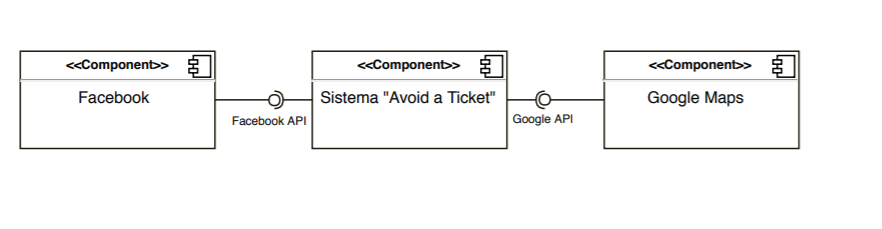
\includegraphics[scale=0.7]{img/Isoriniai_komponentai}
	\caption{Išoriniai komponentai}
	\label{img:Išoriniai komponentai}
\end{figure}

Sistema jungiasi prie Facebook, kai norima prisijungti prie programėlės per Facebook paskyrą.
Sistema jungiasi prie Google Maps, kad būtų matomas žemėlapis, kuriame žymimos kontrolės vietos, rodomi maršrutai ir stotelės (žr. \ref{img:Išoriniai komponentai} pav.).

\subsection{Vidiniai komponentai}
Sistemos dekompozicija pagal vidinius komponentus, jų detalesnio abstrakcijos lygmens sandara.
\begin{figure}[H]
	\centering
	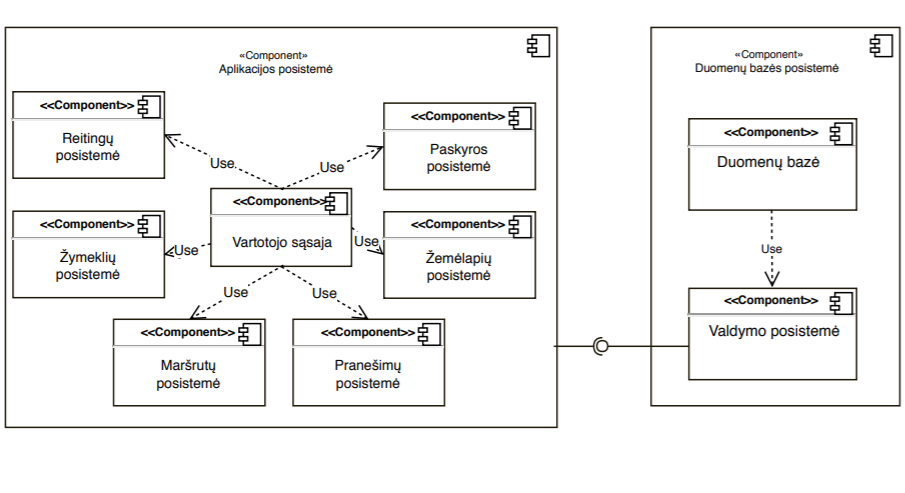
\includegraphics[scale=0.7]{img/Vidiniai_komponentai}
	\caption{Vidiniai komponentai}
	\label{img:Vidiniai komponentai}
\end{figure}

Avoid a Ticket sistemą sudaro dvi posistemės - aplikacijos ir duomenų bazės posistemė. Duomenų bazės posistemėje yra duomenų bazė, kur saugomi sistemos duomenys, ir valdymo posistemė, kuri atlieka duomenų bazių ir kitas užklausas bei jungiasi su aplikacijos posisteme.Aplikacijos posistemėje yra vartotojo sąsaja, kuri pasitelkdama likusias posistemes (paskyros, žemėlapių, pranešimų, maršrutų, žymeklių ir reitingų) ir jų metodus parūpina informaciją vartotojui bei pateikia ją grafiniu būdu (žr. \ref{img:Vidiniai komponentai} pav.).

\subsection{Komponentų išsidėstymas tinkle, jų saugumas}
Skyrelyje pateikiamas sistemos fizinių komponentų išdėstymas tinkle, visa sistemos topologija.

\begin{figure}[H]
	\centering
	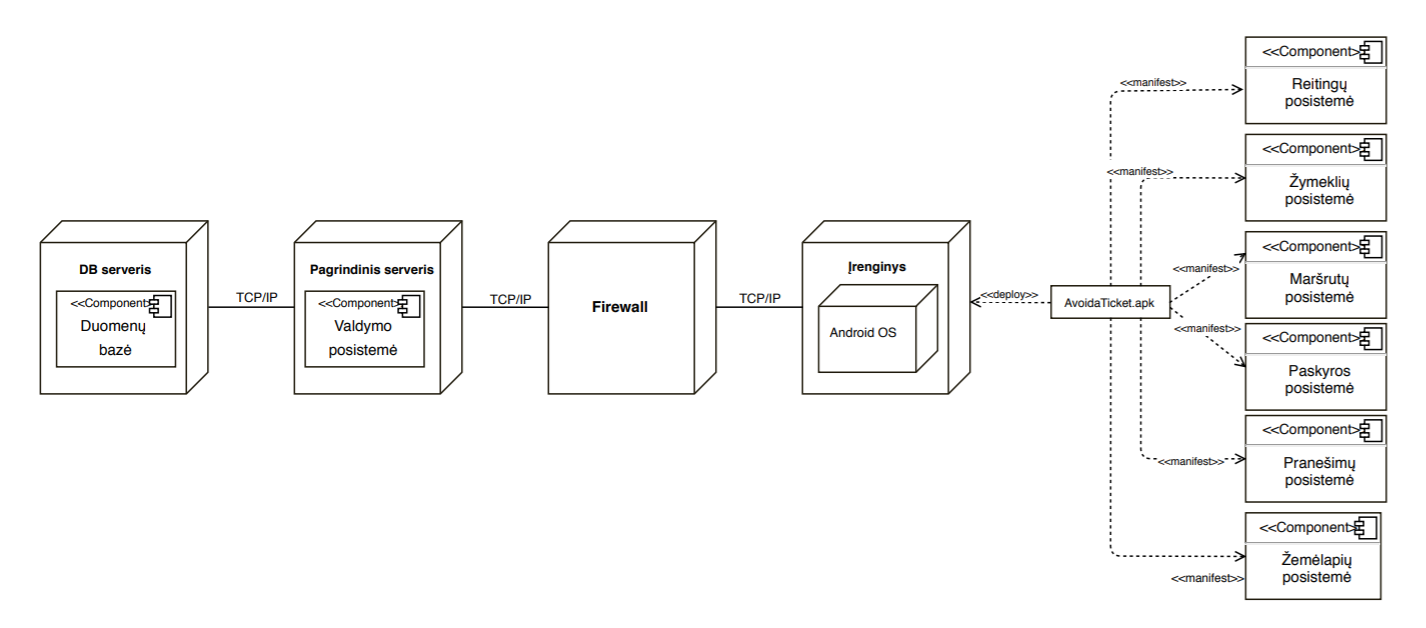
\includegraphics[scale=0.4]{img/Komponentu_issidestymas}
	\caption{Komponentų išsidėstymas}
	\label{img:išsidėstymas}
\end{figure}

Avoid a Ticket sistemoje yra du serveriai, viename jų yra duomenų bazė su duomenimis, kitame – valdymo posistemė, kuri valdo duomenų srautą sistemoje. Taip pat yra
įrenginys su įrašyta android operacine sistema bei Avoid a Ticket aplikacija, kurioje veikia anksčiau minėtos posistemės. Įrenginio naudotojas gali būti administratorius arba klientas. Įrenginiai su pagrindiniu serveriu bei duomenų bazės ir pagrindinis serveriai tarpusavyje siejasi TCP/IP ryšiu, kurio srautą prižiūri „Firewall“ mazgas saugodamas nuo nuotolinių atakų – bandymo išgauti duomenis, kenkėjiškų programų palikimo ar kitos potencialios žalos sistemai (žr. \ref{img:išsidėstymas} pav.).

\subsection{Diegimas ir palaikymas}

Aplikacija talpinama Google „Play Store“ sistemoje, iš kurios kiekvienas asmuo su Android operacinę sistemą palaikančiu įrenginiu gali ją atsisiųsti. Aplikacijos atnaujinimai vyksta taip pat per Google „Play Store“. Vartotojai, pirmą kartą diegiantys programėlę, siunčiasi naujausią tuo metu prieinamą versiją, o atnaujinimo atveju turi galimybę atsisiųsti naujesnę
versiją ir ja pakeisti senesnę.


\sectionnonum{Rastų klaidų sąrašas}
Šiame skyriuje dokumentuojamos visos laboratorinių darbų metu užfiksuotos klaidos
	\begin{enumerate}[itemsep=-2mm]
		\item Struktūriniame esybių modelyje nebuvo Maršruto esybės.
		\item Struktūriniame esybių modelyje Filtro esybė buvo agregacijos ryšiu sujungta su žymekliu.
		\item Struktūriniame dalykinės srities modelyje buvo naudojamos ne tik agregacijos ir generalizacijos.
		\item Netikslus funkcinis reikalavimas, nusakantis, kiek laiko po žymeklio pridėjimo jis yra matomas vartotojams.
		\item Užduočių aprašymuose naudojama ne tik tiesioginė nuosaka.
		\item Struktūriniame esybių modelyje nebuvo atskirų Paskiros ir “Facebook” paskyros esybių.
		\item Nebuvo sunumeruoti paveikslėliai.
		\item Nebuvo funkcinio reikalavimo vartotojo galimybei pasirinkti maršrutą ir tikrinti stoteles pagal jį.
		\item Nebuvo funkcinio reikalavimo vartotojo galimybei filtruoti matomus žymeklius pagal pasirinktą maršrutą.
		\item Netiksliai aprašytas poreikis, kokiu atstumu nuo vartotojo buvimo vietos, jis gali padėti žymeklį.
		\item Neteisingai aprašytas scenarijus “Žemėlapio redagavimas. Vartotojų balsavimas dėl žymeklio teisingumo”
		\item Profilio duomenų redagavimo UC3 panaudojamumo atvejo teksto korekcija - pridėtas naujas alternatyvus scenarijus: nesutampantys slaptažodžiai. 2018-04-17
		\item UC4 panaudojamumo atvejo teksto korekcija - pridėtas naujas alternatyvus scenarijus: tuščias komentaro laukas. 2018-04-17
		\item UC7 teksto patikslinimas: papildoma informacija apie GPS įrenginio dialogo langą. 2018-04-17
		\item UC10 teksto patikslinimas: pridėtas papildomas alternatyvus scenarijus, kai administratorius nori pašalinti tik vieną žymeklį. 2018-04-17
		\item Iš vienos esybės Komentaras sukurtos dvi - Kūrėjo komentaras ir Vartotojo komentaras esybės, reiškiančios du skirtingus sistemos funkcionalumus. 2018-04-17
		\item Pridėti aprašymai dokumento antraštėms. 2018-04-22
		\item Sunumeruotos visos verslo esybės, vartotojo sąsajos langai, panaudojamumo atvejų tekstai. 2018-04-22
		\item Įvade pridėtas naudojamų literatūros sąrašo resursų paminėjimas 2018-04-22

	\end{enumerate}
\sectionnonum{Rezultatai}
Pirmoje ir antroje laboratorinių darbų iteracijose pagal užsakovo poreikius sudaryti funkciniai ir nefunkciniai reikalavimai, nubraižyta dalykinės srities verslo esybių klasių diagrama, kuri papildyta esminiais atributais, surastais braižant robastiškumo diagramas. Pirmoje dalyje nubraižyti vartotojo sąsajos maketai. Taip pat aprašyti visi sistemos panaudojamumo scenarijai, kuriems antroje iteracijoje buvo braižomos robastiškumo diagramos. Antroje iteracijoje taip pat sukurta techninė sistemos architektūra. Trečiosios dokumento iteracijos rezultatas - detalus projekto dizainas, į kurį įeina: operacijų priskyrimas klasėms, techninės architekūros, statinio modelio atnaujinimas, kritinė projekto peržiūra. Taip pat šios dalies metu sukurtas programos prototipas, parašyti testavimo scenarijai ir planai, padengiantys sistemos panaudojamumo atvejus. Visų iteracijų metu pildytas rastų klaidų ir pakeitimų sąrašas.
\sectionnonum{Išvada}
Pirmoje iteracijoje sukurta įvadinė verslo taisyklių logika leidžia toliau sėkmingai detalizuoti sistemos komponentus pereinant į žemesnius abstrakcijos lygius - sistemą galima skaidyti į atskirus verslo esybių modulius ir kiekvieną jų nagrinėti atskirai. Kadangi ICONIX proceso esmė - klaidinga kiekvienos iteracijos įeiga, todėl nereikia baimintis likusių neapibrėžtumų ir abstraktumo - visa tai bus detalizuota kitų laboratorinių darbų metu. Antra iteracija ir jos esminis pagrindas - robastiškumo diagramos - leido „sugaudyti“ likusius panaudojamumo atvejų tekstų dviprasmiškumus, netikslumus ir nepastebėtas naujas esybes. Taigi, apibrėžtas koncepcinis (preliminarus) sistemos modelis, kuris yra tarpinė sritis tarp dalykinės srities analizės ir tikslios techninės architektūros. Trečiosios dalies metu įgyvendintas detalusis projektuojamos sistemos modelis - kiekvienam panaudojamumo atvejui braižytos sekų diagramos leido tinkamai priskirti klasėms elgseną (operacijas), atlikus šį žingsnį galima pradėti įgyvendinti architektūrą rašant kodą, nes žinome esybes ir jų elgesį (OO programavimo pagrindas).

\sectionnonum{Literatūros sąrašas}

\begin{enumerate}[label={[\arabic*]},itemsep=-2mm]
	\item Doc. dr. K. Petrausko Programų Sistemų Inžinerijos kurso konspektai
	\label{petrauskas}
	\item Doug Rosenberg and Matt Stephens - „Use Case Driven Object Modeling with UML Theory and Practice“
	\label{iconix}
	\item UML dokumentacija \url{https://www.tutorialspoint.com/uml/uml_2_overview.htm}
	\label{uml}
	\item OMG UML v.2.5 Dokumentacija diagramoms, žymėjimui
	\label{omguml}
\end{enumerate}

\end{document}
